\documentclass[a4paper,12pt]{jsbook}
\renewcommand{\prechaptername}{Chapter~}
\renewcommand{\postchaptername}{}
\setlength{\textwidth}{\fullwidth}
\setlength{\evensidemargin}{\oddsidemargin}
\usepackage{algorithm}
\usepackage{algpseudocode}
\usepackage{booktabs}  % 用于专业表格线
\usepackage{threeparttable}  % 用于表格注释（如果使用tablenotes）
\usepackage{multirow}  % 用于多行合并（如果需要）
\usepackage{xcolor}
\usepackage{thesis}
\usepackage{makeidx}
\usepackage{amsmath}
\usepackage{txfonts, float}
\usepackage{here}
\usepackage[dvipdfmx]{graphicx}
\usepackage[noto-otc, unicode]{pxchfon}



\begin{document}

% 表紙
\thesis{
\scalebox{}{\bf 2026年度} \\
\scalebox{}{\bf 修\quad 士\quad 論\quad 文}
}
\date{2026年1月9日}
\title{
    \vspace{1.2zh}
    \scalebox{0.9}{RNA 3D Structure Prediction by Diffusion Structural Model}\\
    \scalebox{0.9}{（拡散構造モデルによるRNA立体構造予測）}
}
\teacher{\quad 浅井\quad 潔\quad 教授}
\organization{
    東京大学大学院新領域創成科学研究科\\
    メディカル情報生命専攻}
\author{
\scalebox{1}{崔 \quad 宇軒} \\
\scalebox{1}{Cui, Yuxuan}
}

\maketitle

% 前書き
\chapter*{Abstract}
\thispagestyle{empty}
RNA molecules play essential biological roles whose functions are critically determined by their three-dimensional (3D) structures. However, experimental determination of RNA 3D structures remains challenging, and existing computational approaches still struggle to achieve accurate, generalizable predictions across diverse RNA families and lengths. In particular, deterministic deep learning models often suffer from limited robustness to conformational heterogeneity, length scaling, and RNA-specific geometric constraints.

In this thesis, we propose Diffold, a diffusion-based generative framework for RNA 3D structure prediction. Diffold integrates (i) the evolutionary and geometric representations produced by the RhoFold+ backbone, (ii) structural priors derived from the large-scale RNA language model RNA-FM, and (iii) an Elucidated Diffusion Model (EDM) formulation to generate all-atom RNA coordinates through iterative denoising. A hierarchical token–atom denoising architecture is employed to simultaneously capture long-range residue-level dependencies and local atomic geometry, enabling physically plausible structure generation in Cartesian coordinate space.

Diffold is evaluated on the combined CASP16 RNA targets and the RNA-Benchmark dataset. Across all major metrics, Diffold consistently outperforms the strong baseline RhoFold+. Specifically, Diffold reduces RMSD from 3.85 $\text{\AA}$ to 2.29 $\text{\AA}$ and improves TM-score from 0.309 to 0.585, indicating substantially improved global fold recovery. Additional gains are observed in GDT-TS and lDDT, together with a marked reduction in steric clashes, reflecting enhanced local geometric consistency and physical plausibility. Further analyses demonstrate that Diffold exhibits weaker dependence on training-set structural similarity and improved robustness to increasing sequence length, suggesting stronger generalization than deterministic backbone-based methods.

Finally, we show that a lightweight AMBER-based relaxation step effectively corrects local covalent-geometry artifacts, such as elongated O3′–P bonds, without materially affecting global accuracy. Overall, these results indicate that diffusion-based generative modeling, when conditioned on rich RNA-specific representations, provides a promising and extensible strategy for accurate and generalizable RNA 3D structure prediction.
\frontmatter
\renewcommand{\contentsname}{Contents}
\renewcommand{\bibname}{References} 
\renewcommand{\refname}{References}
\tableofcontents

% 本文
\mainmatter

\chapter{Introduction}

Ribonucleic acid (RNA) performs diverse and essential biological functions, including gene regulation, catalysis, ligand sensing, viral genome packaging, and acting as a structural scaffold within ribonucleoprotein complexes. These functions critically depend on the ability of RNA molecules to fold into well-defined three-dimensional (3D) conformations, involving complex long-range tertiary interactions, non-canonical base-pair geometries, backbone torsion-angle patterns, sugar-pucker states, and metal-ion–mediated contacts. Understanding RNA 3D structure is therefore fundamental not only to elucidating molecular mechanisms, but also to enabling a wide range of biomedical applications such as RNA-targeted therapeutics, siRNA design, ribozyme engineering, gene-editing systems, and mRNA vaccine development.

Experimental techniques such as X-ray crystallography, nuclear magnetic resonance (NMR) spectroscopy, and cryo-electron microscopy (cryo-EM) can provide high-resolution RNA structures, but their applicability is limited. Many RNAs are too flexible to crystallize, NMR analysis is constrained by molecular size, and cryo-EM is mainly suited to large complexes rather than small or moderately sized RNAs. Chemical probing approaches, including SHAPE, DMS, and PARS, offer valuable constraints on secondary structure but cannot directly reveal atomic-resolution tertiary conformations. Consequently, the number of experimentally solved RNA structures remains small compared to proteins, which restricts the availability of high-quality data for training and benchmarking computational models of RNA 3D structure.

Before the rise of deep learning, computational RNA structure prediction relied primarily on thermodynamic modeling and free-energy minimization. Classical algorithms such as MFold, ViennaRNA (RNAfold), and RNAstructure employ dynamic programming to estimate minimum free-energy secondary structures under the Turner nearest-neighbor parameters, and have been widely used for predicting base-pairing patterns and analyzing thermodynamic ensembles\cite{Zuker2003Mfold, Lorenz2011ViennaRNA, Reuter2010RNAstructure}. Although extensions such as partition-function calculations and stochastic context-free grammars allow ensemble-based reasoning and base-pair probability estimation, these methods fundamentally operate at the secondary-structure level and cannot explicitly capture tertiary interactions, complex motifs, pseudoknots (without substantial simplification), or detailed backbone geometry. As a result, traditional thermodynamic approaches provide only limited insight into the full 3D conformational landscape of RNA molecules.

In recent years, deep learning has substantially reshaped RNA secondary structure prediction. Methods such as SPOT-RNA, MXfold2, and UFold learn base-pairing rules directly from data, integrating convolutional or transformer-based architectures with thermodynamic priors or image-like representations of base-pair matrices, and consistently outperform classical thermodynamic models on within-family and cross-family benchmarks\cite{Singh2019SPOTRNA, Sato2021MXfold2, Fu2022UFold}. These approaches demonstrate that data-driven models can capture non-trivial base-pairing patterns, including non-canonical and long-range interactions, thereby providing more accurate secondary structure inputs for downstream 3D modeling.

A major class of methods for RNA 3D structure prediction is template-assembly–based modeling. The Rosetta FARFAR and FARFAR2 frameworks assemble RNA structures by recombining experimentally derived or computationally sampled fragments and refining them with an all-atom energy function\cite{Watkins2020FARFAR2}. These methods have shown strong performance in RNA-Puzzles challenges and can produce high-quality models for certain families, especially when homologous templates or motifs are available. Similarly, RNAComposer employs module-based assembly using a library of recurrent structural motifs, enabling rapid generation of coarse-grained 3D structures that approximate native folds\cite{Biesiada2016RNAComposerProtocol}. However, fragment-based approaches depend heavily on template availability and struggle with novel motifs, large conformational variability, and RNAs lacking homologous structures.

And another important class of methods for RNA 3D structure prediction is deep-learning-based modeling. DRfold integrates end-to-end learning of local frames with geometric restraints to assemble RNA 3D structures, combining learned potentials with energy-based refinement\cite{Li2023DRfold}. trRosettaRNA extends the successful trRosetta framework from proteins to RNA, using transformer networks to predict 1D and 2D geometric features such as orientations, distances, and contacts, followed by energy minimization to obtain full-atom models\cite{Wang2023trRosettaRNA}. More recently, RhoFold+ leverages an RNA language model pretrained on tens of millions of RNA sequences together with geometric deep learning modules to achieve state-of-the-art accuracy on RNA-Puzzles and CASP benchmarks\cite{Shen2024RhoFoldPlus}. Although these models substantially improve over classical and homology-based approaches, they still face difficulties in capturing highly flexible regions, rare non-canonical motifs, backbone torsion-angle distributions, and the multiple conformational states that many RNAs can adopt.

The transformative success of AlphaFold2 (AF2) in protein structure prediction has further stimulated efforts to adapt AF2-like architectures to RNA\cite{Jumper2021AlphaFold}. AF2 introduced attention-based pair representations, iterative refinement, and end-to-end differentiable structure modules, enabling near-experimental accuracy for many protein targets. AlphaFold3 (AF3) subsequently incorporated a diffusion-based architecture and unified the modeling of proteins, nucleic acids, small molecules, and other components in macromolecular complexes\cite{Abramson2024AlphaFold3}. However, when applied to RNA-only targets, AF3 and AF2-style pipelines still exhibit limited accuracy: several recent evaluations report unrealistic sugar-pucker conformations, incorrect non-canonical base-pair geometries, and frequent steric clashes in the RNA backbone, reflecting the fact that these models are trained predominantly on protein-centric datasets and are not explicitly optimized for RNA-specific geometric constraints.

In parallel, two methodological developments have opened new possibilities for RNA modeling: RNA language models and diffusion-based generative models. RNA foundation models such as RNA-FM learn contextual representations from tens of millions of unannotated RNA sequences via self-supervised learning and have been shown to capture structural and functional information useful for downstream tasks\cite{Chen2022RNAFM}. RNABERT and related models further demonstrate that pretraining on nucleotide sequences can encode base-level features relevant to clustering and structural alignment\cite{Akiyama2022RNABERT}. On the generative side, diffusion models have emerged as a powerful framework for molecular structure generation. Recent work on protein structure generation via folding diffusion and related approaches shows that diffusion models can produce realistic protein backbones and conformational ensembles, while maintaining physical plausibility through carefully designed noise processes and geometric parameterizations\cite{Yim2024DiffusionReview, Wu2024FoldingDiffusion}. These advances suggest that combining RNA-specific language model embeddings with diffusion-based generative modeling may provide a flexible and physically grounded strategy for RNA 3D structure prediction.

In conclusion, existing experimental and computational approaches still fall short of providing accurate and generalizable RNA 3D structure predictions across diverse families and sequence lengths. Thermodynamic methods are restricted to the secondary structure, discriminative deep learning models struggle with conformational heterogeneity and rare tertiary motifs, and AF2-style architectures are limited by protein-centric training data and RNA-specific geometric differences. Motivated by these challenges and by recent progress in RNA language models and diffusion-based generative modeling, this study aims to develop a diffusion structural model tailored specifically for RNA 3D structure prediction. The proposed framework is designed to integrate RNA language model embeddings as structural priors and to explore RNA conformational space through a diffusion process that respects RNA geometry and chemical constraints, with the ultimate goal of improving geometric accuracy, capturing diverse tertiary motifs, and enhancing generalization across RNA families.

\bigskip

In this thesis, we propose a diffusion-based generative model for RNA three-dimensional structure prediction. The model builds upon the geometric backbone of RhoFold+, integrates structural priors provided by the large-scale RNA language model RNA-FM, and employs the Elucidated Diffusion Model (EDM) as the core generative mechanism to construct physically plausible RNA 3D conformations\cite{Karras2022EDM}.

\noindent{The main contributions of this thesis are:}

\begin{enumerate}
    \item {A diffusion-based generative model Diffold for RNA tertiary structure prediction}, 
          integrating RNA-FM structural priors, the RhoFold+ geometric backbone, and 
          the Elucidated Diffusion Model (EDM) for physically consistent structure generation.

    \item {A full RNA-oriented diffusion architecture} featuring:
    \begin{itemize}
        \item An EDM-based structural generation module;
        \item An RNA-specific denoising network designed to incorporate atomic chemical features;
    \end{itemize}

    \item {Comprehensive experimental validations} on CASP16 RNA targets and the RNA-Benchmark dataset:
    \begin{itemize}
        \item Systematic comparisons against state-of-the-art RNA tertiary structure predictors;
        \item Evaluation of the effects and limits of diffusion-based generative modeling for RNA structures.
    \end{itemize}
\end{enumerate}

\bigskip

\noindent{The remainder of this thesis is organized as follows:}

\begin{itemize}
    \item{Chapter 2} presents the overall methodology, including RNA-FM sequence representation, 
          the RhoFold+ backbone, the Elucidated Diffusion Model, and the RNA-specific denoising architecture.

    \item{Chapter 3} describes the datasets used in this study (CASP16 and RNA-Benchmark)\cite{Ludaic2025limits}, 
          baseline models, evaluation metrics, and experimental settings.

    \item{Chapter 4} provides experimental results, comparisons with existing approaches, 
          and detailed analyses of representative prediction cases.

    \item{Chapter 5} concludes the thesis and discusses limitations and future directions, 
          including potential advancements toward more generalizable RNA generative models.
\end{itemize}

\chapter{Methods}

\begin{figure}
    \centering
    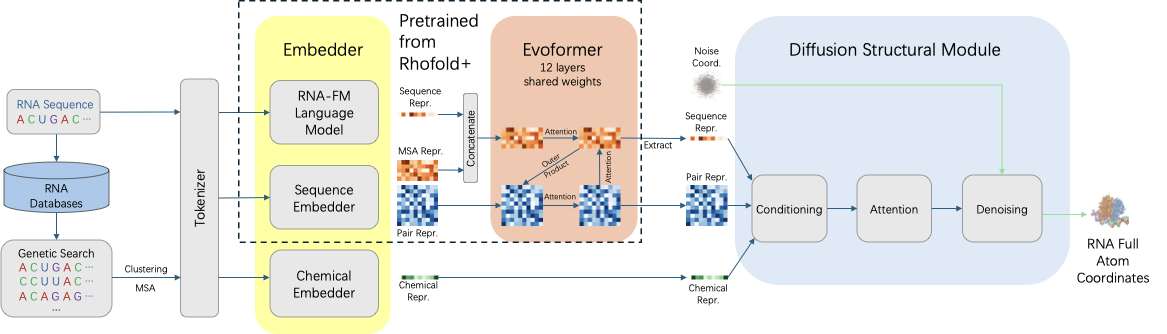
\includegraphics[width=1\linewidth]{img/Architecture.png}
    \caption{Overview of the Diffold framework}
    \label{fig:architecture}
\end{figure}

\section{MSA Feature Generation}
In this study, the model uses multiple sequence alignment (MSA) features to capture evolutionary information among RNA sequences. For each target RNA sequence, we perform a remote BLASTN search against the NCBI nucleotide (nt) database using the BLAST “QBlast” Common URL API provided by NCBI. The QBlast API is an HTTP-based programmatic interface to the NCBI BLAST servers, allowing automated submission of search queries, retrieval of job status, and downloading of alignment results without manual intervention. In our implementation, we adopt the “Put/Get” workflow of the Common URL API to submit each query sequence, parse the returned results, and rank the obtained homologous sequences based on E-value and bit score\cite{altschul1990blast, altschul1997gappedblast}. Due to hardware memory limitations, we retain up to 250 non-redundant homologous sequences as the maximum MSA depth. In contrast to models such as AlphaFold2 and RhoFold+, which rely on different MSA construction tools and databases, our approach uses QBlast for remote retrieval\cite{Jumper2021AlphaFold}. Following sequence retrieval, we apply the same alignment and feature-construction procedures as RhoFold+ to build the MSA, from which we extract per-position MSA profiles and pairwise co-evolutionary features as input to the Rhoformer backbone. Compared to maintaining a local BLAST database, using QBlast simplifies deployment and ensures continuous access to the most up-to-date NCBI nt database.

\section{Embedder}

Our model adopts a token-based feature embedding strategy, where each token corresponds to a nucleotide residue in the RNA sequence. The embedding module consists of two core components: token embedder and atom embedder.
\subsection{Token Embedder}
\subsubsection{MSA Embedder}

This module receives a multiple sequence alignment (MSA) as input, with shape $\mathbb{R}^{B \times K \times L}$, where $B$ denotes the batch size, $K$ the number of aligned sequences, and $L$ the sequence length. A learnable token embedding layer maps discrete nucleotide tokens into a 256-dimensional continuous vector space. To capture positional information, we apply a learned positional embedding that supports maximum sequence lengths up to 4096.

To construct pairwise representations, we adopt an outer-product–style strategy: given a sequence embedding $e \in \mathbb{R}^{L \times d}$, the pairwise representation is formed by concatenating embeddings at positions $i$ and $j$, namely
$p_{ij} = [\, e_i \oplus e_j \,],$
where $\oplus$ denotes the concatenation operation. A linear projection followed by 2D sinusoidal positional encoding yields the final pairwise feature tensor $\mathbf{Z} \in \mathbb{R}^{L \times L \times 128}$.

Meanwhile, we use the pretrained RNA language model RNA-FM to enhance representational capacity\cite{Chen2022RNAFM}. RNA-FM is based on a 12-layer Transformer architecture and is pretrained on large-scale RNA sequence corpora, providing a 640-dimensional single-sequence representation $\mathbf{S}_{\text{RNA-FM}}$. Through feature concatenation and linear dimensionality reduction, we fuse RNA-FM features with MSA-derived embeddings:
$$\mathbf{M} = \text{Linear}\left([\mathbf{M}_{\text{MSA}} \oplus \mathbf{S}_{\text{RNA-FM}}]\right)$$

\subsubsection{Recycling Embedder}
Inspired by the recycling mechanism of AlphaFold2, this module incorporates predictions from the previous iteration as additional input for the current iteration. Given the single representation $\mathbf{s}^{(t-1)} \in \mathbb{R}^{L \times 256}$, pair representation $\mathbf{z}^{(t-1)} \in \mathbb{R}^{L \times L \times 128}$, and the predicted C1′ atomic coordinates $\mathbf{x}^{(t-1)}_{\text{C1}'} \in \mathbb{R}^{L \times 3}$ from iteration $t-1$, the recycling embedder first converts coordinates into a distance-histogram representation:
$$d_{ij} = \text{OneHot}\bigl(\|\mathbf{x}_i - \mathbf{x}_j\|_2,\ \text{bins} = [2, 22]\ \text{\AA}\bigr)$$
The 15-dimensional binned distances are then projected to 128 dimensions via a linear layer and added to the normalized pairwise features. The MSA features are layer-normalized and added to the first row of the current MSA representation.
This design allows the model to inject geometric constraints across recycling iterations, enabling progressive refinement of predicted structures.

\subsection{Atom Embedder}


Unlike traditional token-level representations, our model adopts an atom-level embedding strategy to capture finer-grained intramolecular interactions. This module follows Algorithm 2 of AlphaFold3, transforming raw atomic coordinates into multi-scale hierarchical representations.

  
\subsubsection{Atomic Feature Initialization}

Given the atomic coordinates $\mathbf{a} \in \mathbb{R}^{N_{atom} \times 3}$ and atom-pair relations $\mathbf{p} \in \mathbb{R}^{N_{atom} \times N_{atom} \times 5}$ (where  is the total number of atoms), we apply bias-free linear layers to map inputs into the embedding space: $$\mathbf{A}^{(0)} = W_a \mathbf{a},\quad \mathbf{P}^{(0)} = W_p \mathbf{p},$$
where atomic features are 128-dimensional and pairwise features are 16-dimensional.

  
\subsubsection{Atom Representation Conditioning}
To enhance expressiveness of pairwise features, we introduce a node–edge conditioning mechanism. For each atomic feature, an MLP produces a modulation signal:

$$\mathbf{c} = \text{ReLU}\left(\text{Linear}\left(\text{LayerNorm}(\mathbf{A}^{(0)})\right)\right) \in \mathbb{R}^{N_{atom} \times 32}$$

The vector $\mathbf{c}$ is split into row- and column-wise modulation terms $\mathbf{c}_{\text{row}}$ and $\mathbf{c}_{\text{col}}$ (each 16-dimensional), which are added to the windowed pairwise features, enabling atomic properties to modulate atom–atom interactions.

  
\subsubsection{Windowed Atomic Transformer}

To support large molecular systems that may contain thousands of atoms, we apply a sliding-window mechanism that partitions the atom sequence into $N_w$ windows of size $w = 27$. Within each window, a Diffusion Transformer layer performs self-attention:

$$\mathbf{A}^{(l+1)} = \text{DiffusionTransformer}^{(l)}\bigl( \mathbf{A}^{(l)},\ \text{single} = \mathbf{A}^{(l)},\ \text{pairwise} = \mathbf{P}^{(l)} \bigr),$$

for $l \in {1, 2, 3}$. Each layer contains four attention heads and learns local atomic interaction patterns.

The windowing strategy reduces computational complexity from $O(N_{atom}^2)$ to $O(N_{atom} \cdot w)$, making it feasible to model large ligand–RNA complexes.

  
\subsubsection{Atom-to-Token Pooling}

Since functional units of biomolecules typically act at the residue (token) level rather than the atom level, we aggregate atom-level embeddings into token-level features via masked average pooling.
Let $N_{\text{atom}}$ denote the number of atoms and $L$ the number of tokens (residues).
We define an atom mask $\mathbf{m}_a \in \{0,1\}^{N_{\text{atom}}}$ and an atom-to-token assignment vector
$\mathbf{g} \in \{1,\dots,L\}^{N_{\text{atom}}}$, where $g_j$ indicates the token index to which atom $j$ belongs.
Accordingly, the set of atoms assigned to token $i$ is
\[
\mathcal{A}(i) = \{\, j \in \{1,\dots,N_{\text{atom}}\} \mid g_j = i \,\}.
\]
Given atom embeddings $\mathbf{h}^{\text{atom}}_j \in \mathbb{R}^{d_a}$, the pooled token feature $\mathbf{T}_i \in \mathbb{R}^{d_a}$ is computed as
\[
\mathbf{T}_i
= \frac{\sum_{j \in \mathcal{A}(i)} m_a[j]\;\mathbf{h}^{\text{atom}}_j}
       {\sum_{j \in \mathcal{A}(i)} m_a[j] + \varepsilon},
\]
where $\varepsilon>0$ is a small constant to avoid division by zero when a token has no valid atoms after masking.


  

The embedder outputs a named tuple consisting of:

1. $\mathbf{A}^{B \times N_{atom} \times 128}$ — atom-level features,
    
2. $\mathbf{P}^{B \times N_w \times w \times 16}$ — windowed pairwise features, $N_w$ denotes the number of windows.
    

This hierarchical design enables the model to capture molecular interactions at atomic resolution while performing efficient global reasoning at the token level, achieving a balance between computational efficiency and modeling fidelity.

\section{Rhoformer}

We adopt the Rhoformer architecture from RhoFold+ as the backbone network\cite{Shen2024RhoFoldPlus}, which is responsible for integrating evolutionary information with structural constraints. The module takes as input the MSA representation $\mathbf{M} \in \mathbb{R}^{B \times K \times L \times 256}$ and the pair representation $\mathbf{Z} \in \mathbb{R}^{B \times L \times L \times 128}$, and updates them through 12 stacked Rhoformer blocks.

  

Each block consists of two update stages.

(1) MSA update stage. Row attention with pair bias and column attention are applied to capture both intra-sequence dependencies and cross-sequence coevolutionary signals.

(2) Pair update stage. The module performs outer-product mean, triangle multiplicative updates, triangle attention, and a transition feed-forward network, which collectively project information from the MSA space into the residue-pair space and strengthen geometrical consistency. Bidirectional information flow between the MSA and pair representations is maintained through pair biases and outer-product operations.

After 12 update blocks, the single-sequence representation is extracted from the first row of the MSA (corresponding to the query sequence) as

$$\mathbf{S} = \text{Linear}(\mathbf{M}[0]) \in \mathbb{R}^{B \times L \times 256},$$

which is then fed, together with the refined pair representation, into the subsequent Structure Module. All submodules employ residual connections and layer normalization to stabilize the training of deep networks. To reduce memory consumption for long sequences, we additionally apply gradient checkpointing and a dynamic chunking mechanism.

\section{Diffusion Structural Module}

Diffusion models are a class of generative models grounded in stochastic differential processes\cite{sohldickstein2015diffusion, ho2020ddpm}. Their core idea is to gradually perturb the data distribution into an isotropic Gaussian distribution through a forward noising process, and to learn a reverse denoising process that progressively recovers samples consistent with the target distribution starting from random noise. Unlike conventional direct regression-based generative models, diffusion models represent complex high-dimensional distributions through multi-step iterative refinement, which has demonstrated superior stability and diversity in structural generation tasks.

In the task of RNA three-dimensional structure prediction, we treat the molecular 3D atomic coordinates as the data to be modeled. Let the ground-truth atomic coordinates be denoted as  $\mathbf{x}_0 \in \mathbb{R}^{N_{atom} \times 3}$,  where $N_{atom}$ represents the total number of atoms in the molecule.

The diffusion process can be conceptually divided into two stages, forward diffusion process and reverse denoising process.

The forward diffusion process gradually corrupts the original data by adding Gaussian noise, mapping clean samples into a family of noisy distributions. For any continuous noise level $\sigma > 0$, the forward process is defined as

$$  
\mathbf{x}_\sigma = \mathbf{x}_0 + \sigma \boldsymbol{\epsilon},  
\quad \boldsymbol{\epsilon} \sim \mathcal{N}(\mathbf{0}, \mathbf{I}),  
$$

where $\mathbf{x}_\sigma$ denotes the perturbed coordinates at noise scale $\sigma$. As $\sigma$ increases, the data distribution progressively approaches an isotropic Gaussian distribution; in the limit $\sigma \to \infty$, the samples contain almost no structural information. This continuous formulation of noise injection avoids the explicit Markov chain construction used in discrete-time diffusion models, providing a convenient foundation for designing stable reverse processes.


The reverse denoising process makes the generative capability of diffusion models, which aims to progressively recover the original data $\mathbf{x}_0$ from noisy samples $\mathbf{x}_\sigma$. This process can be interpreted as iterative denoising in noise-scale space, moving from higher noise levels toward lower ones.

In theory, the reverse process corresponds to a conditional distribution
$$  
p(\mathbf{x}_{\sigma'} \mid \mathbf{x}_\sigma),  
\quad \sigma' < \sigma,  
$$
whose exact form is generally intractable. In practice, this distribution is approximated using a neural network.

Specifically, diffusion models train a parameterized denoising network $\mathbf{D}_\theta$ that predicts a denoised estimate given noisy coordinates and the corresponding noise level:

$$  
\hat{\mathbf{x}}_0 = \mathbf{D}_\theta(\mathbf{x}_\sigma, \sigma).  
$$

This network effectively learns the conditional expectation of the data distribution across noise scales, enabling structure correction at arbitrary noise levels.

\begin{figure}
    \centering
    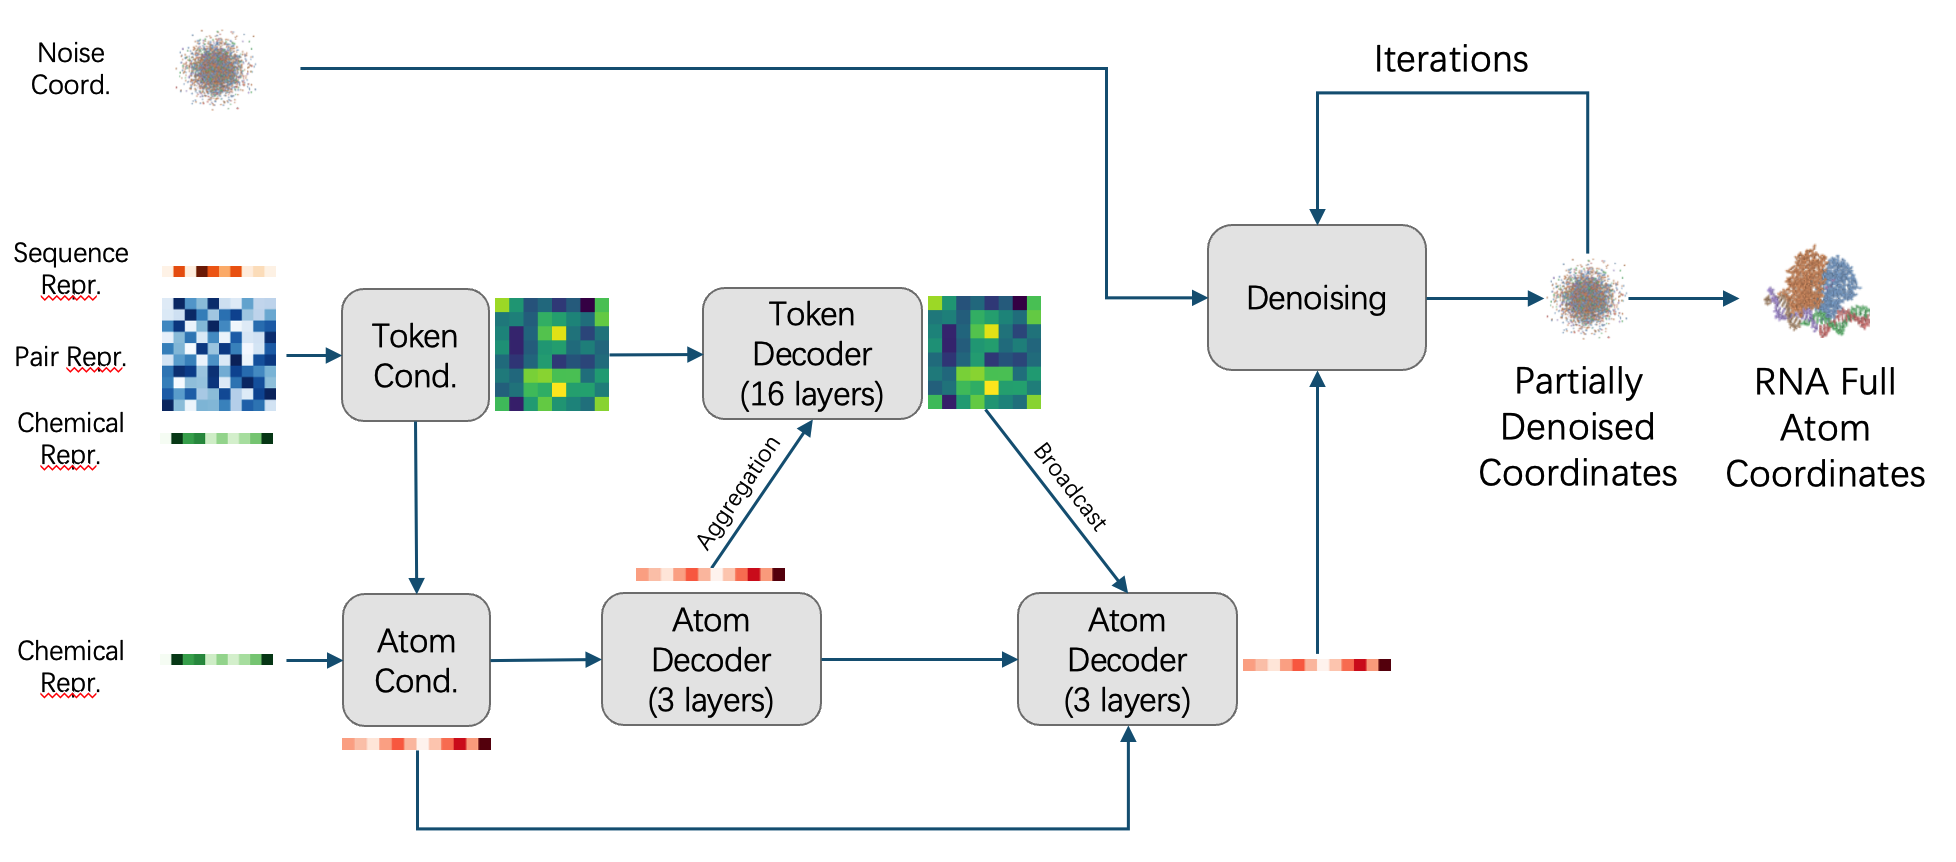
\includegraphics[width=1\linewidth]{img/Diffusion_module.png}
    \caption{Overview of the diffusion structural module. Noisy atom coordinates are iteratively refined by a token-level decoder and an atom-level decoder with bidirectional aggregation and broadcasting. Sequence/pair representations and chemical features are injected via token/atom conditioning to produce full-atom RNA coordinates.}
    \label{fig:diffusion module}
\end{figure}

\subsection{Conditional Diffusion Modeling}

In RNA structure prediction, the generated three-dimensional conformations must be consistent with given biological conditions, such as sequence information, evolutionary constraints, and chemical structure features. Therefore, the denoising network is formulated as a conditional model:

$$  
\hat{\mathbf{x}}_0 = \mathbf{D}_\theta(\mathbf{x}_\sigma, \sigma \mid \mathcal{C}),  
$$

where $\mathcal{C}$ denotes the set of all conditional inputs, including residue-level representations, atomic features, atom-pair relationships, and masking information.

During training, the model minimizes the discrepancy between predicted and ground-truth coordinates across different noise levels, learning to leverage conditional information to progressively remove noise and recover physically plausible 3D structures. During inference, the model starts from Gaussian noise and iteratively applies the reverse denoising process to generate the final structure.


\subsection{Elucidated Diffusion Model（EDM)}


In this study, we adopt the Elucidated Diffusion Model (EDM) framework proposed by Karras et al. to perform diffusion modeling of atomic coordinates\cite{Karras2022EDM}. Compared to conventional DDPM-style approaches, EDM treats the continuous noise level $\sigma$ as a core variable and unifies learning across different noise scales via a preconditioning mechanism, leading to improved training stability and sampling efficiency.

During training, noisy samples are constructed from the ground-truth coordinates $\mathbf{x}_0$ as

$$  
\mathbf{x} = \mathbf{x}_0 + \sigma \boldsymbol{\epsilon}, \qquad \boldsymbol{\epsilon} \sim \mathcal{N}(\mathbf{0}, \mathbf{I}),  
$$

and the model learns a noise-conditioned denoising mapping that exhibits consistent recovery capability across multiple noise scales.

\subsection{Token–Atom Hierarchical Denoising Architecture}

The core of the diffusion model is the denoising network $\mathcal{F}_\theta$, whose objective is to recover physically plausible molecular conformations from noisy structures under a given noise level. To address the hierarchical nature of RNA structures—characterized by both atom-level local geometric constraints and residue-level long-range interactions—we employ a Token–Atom hierarchical denoising architecture inspired by AlphaFold3. This design models structural information at multiple scales, achieving a balance between computational efficiency and modeling accuracy.

Biomolecular structures such as RNA and proteins exhibit intrinsic hierarchy. At the microscopic scale, bond lengths, bond angles, and non-bonded interactions govern local geometric stability; at higher levels, residue stacking, secondary structure elements, and long-range contacts determine the global folding topology. Performing global self-attention over all atomic pairs incurs a computational complexity of $O(M^2)$, which is infeasible for medium- to large-scale RNA molecules in terms of both computation and memory.

To overcome this limitation, we decompose the denoising process into two cooperating levels:  
(1) an atom level, responsible for modeling local geometry and short-range interactions;  
(2) a token (residue) level, responsible for modeling long-range dependencies and global structural patterns.

Information exchange between these two levels is achieved through atom-to-token aggregation and token-to-atom broadcasting, enabling the model to retain atomic precision while efficiently capturing global structural constraints.

\subsubsection{Token Decoder}

At the token level, a global Transformer is used to model long-range residue–residue interactions. The Token Transformer consists of 16 Transformer blocks (each with 16 attention heads). Its inputs include the pooled token representations $\mathbf{T}_{\text{input}} \in \mathbb{R}^{L \times d_t}$, residue-level single representations $\mathbf{s}_{\text{single}} \in \mathbb{R}^{L \times d_s}$, and residue-pair representations $\mathbf{z}_{\text{pair}} \in \mathbb{R}^{L \times L \times d_p}$ from the backbone network:

$$  
\mathbf{T} =  
\mathrm{TokenTransformer}\left(  
\mathbf{T}_{\text{input}}, \mathbf{s}_{\text{single}}, \mathbf{z}_{\text{pair}}  
\right)  
$$

The attention mechanism is defined as

$$  
\mathrm{Attention}(\mathbf{Q}, \mathbf{K}, \mathbf{V})
\mathrm{softmax}\left(  
\frac{\mathbf{Q}\mathbf{K}^\top}{\sqrt{d_k}} + \mathbf{B}_{\text{pair}}  
\right)\mathbf{V},  
$$

where $\mathbf{B}_{\text{pair}}$ is a learned attention bias obtained via linear projection of the residue-pair features $\mathbf{z}_{\text{pair}}$. At the token level, the computational complexity is $O(L^2 \cdot d_t)$, which is efficient due to $L \ll N_{atom}$.


\subsubsection{Token-to-Atom Broadcasting}


To propagate global structural information back to the atomic level, each token representation is broadcast to all atoms belonging to that residue and combined with the atom encoder output via a residual connection:

$$  
\mathbf{h}_{\text{atom}}^{\text{dec}} =  
\mathrm{Broadcast}(\mathbf{T}) + \mathbf{h}_{\text{atom}}^{\text{enc}}  
$$

This operation preserves local geometric information while injecting global residue-level constraints.


\subsubsection{Atom Decoder}

In the final stage, denoising is performed again at the atomic level. The atom decoder mirrors the atom encoder architecture, employing windowed self-attention and consisting of three Transformer blocks:

$$  
\mathbf{h}_{\text{atom}}^{\text{final}} =  
\mathrm{AtomDecoder}\left(  
\mathbf{h}_{\text{atom}}^{\text{dec}}, \mathbf{z}_{\text{atom-pair}}  
\right).  
$$

Finally, a linear projection predicts the atomic coordinate updates:

$$  
\Delta \mathbf{x} =  
\mathrm{Linear}(\mathbf{h}_{\text{atom}}^{\text{final}})  
\in \mathbb{R}^{M \times 3}.  
$$

This hierarchical denoising architecture enables the model to recover local geometry at atomic resolution while capturing global folding patterns at the token level, forming a key design that makes diffusion-based modeling effective for RNA three-dimensional structure generation.


\subsection{Conditional Information and Time Embedding}

To ensure consistency between the generated structures and the input sequence, evolutionary information, and chemical constraints, the denoising network $\mathbf{F}_\theta$ incorporates multi-modal conditioning. The conditional inputs used in the diffusion module include atomic features $\mathbf{h}_{\mathrm{atom}} \in \mathbb{R}^{M \times d_a}$, atom-pair features $\mathbf{h}_{\mathrm{pair}} \in \mathbb{R}^{M \times M \times d_{ap}}$, residue-level representations $\mathbf{s} \in \mathbb{R}^{L \times d_s}$, residue-pair representations $\mathbf{z} \in \mathbb{R}^{L \times L \times d_p}$, and atomic validity masks $\mathbf{m}_{\mathrm{atom}} \in {0,1}^{M}$, where $L$ denotes the number of residues.

The noise level $\sigma$ is transformed via $c_{\mathrm{noise}}(\sigma)$ and injected into the network using sinusoidal positional encoding to represent diffusion “time”:

$$  
\mathbf{t}_{\mathrm{emb}}(\sigma)
=
\Big[  
\sin(\omega_k, c_{\mathrm{noise}}(\sigma)),  
\cos(\omega_k, c_{\mathrm{noise}}(\sigma))  
\Big]_{k=1}^{K}  
$$

This time embedding enables the network to learn noise-level–dependent denoising strategies and, together with multi-modal conditioning, determines the direction of structural updates.

\section{Post-processing}

Because the diffusion model directly generates all-atom coordinates in three-dimensional space, its optimization objective primarily focuses on global geometric consistency and distribution matching, rather than explicitly enforcing ideal covalent bond lengths and bond angles. As a result, in a subset of predicted structures, we observed abnormally elongated O3′–P phosphodiester bonds along the RNA backbone, which manifest as apparent chain breaks in the predicted RNA structures.

To correct these local geometric inconsistencies and to ensure the physical plausibility of the generated conformations, we introduce an additional molecular mechanics–based relaxation step as a post-processing procedure after diffusion-based structure generation. Specifically, we employ the AMBER relax protocol provided by the AMBER molecular simulation package to perform energy minimization on the predicted RNA structures\cite{case2023ambertools}. Under a fixed molecular topology, this relaxation procedure adjusts covalent bond lengths, bond angles, dihedral angles, and non-bonded interactions according to classical force-field parameters, thereby effectively repairing abnormal O3′–P bond lengths and resolving severe geometric clashes.

It is important to emphasize that this relaxation step is applied exclusively as a post-processing correction and does not participate in model training or structure generation. We quantitatively compared structural evaluation metrics, including RMSD and TM-score, before and after relaxation, and observed that this procedure does not introduce a significant change in overall prediction accuracy. Its primary role is to improve the physical realism and chemical integrity of the generated RNA conformations, ensuring that the final outputs are more consistent with experimentally observed molecular structures.


\chapter{Datasets and Experiments}

\section{Dataset}
\subsection{Training Data}

To ensure comparability with existing methods and to minimize performance differences caused by dataset factors, we used the same data source and construction strategy as RhoFold+ for training\cite{Shen2024RhoFoldPlus}. Specifically, experimentally resolved single-chain RNA structures were screened from the Protein Data Bank (PDB) and curated as supervised signals. In the original RhoFold+ study, available RNA structures in the PDB were aggregated using the BGSU representative sets (version 2022-04-13). In this thesis, the training set is kept identical to the publicly released RhoFold+ training data, with the primary goal of enabling fair comparisons with RhoFold+ and related backbone-based approaches.

\subsection{Test Data}

For evaluation, we used two public test sources: the RNA-benchmark dataset and the CASP16 RNA targets. CASP16 included nucleic-acid categories such as RNA/DNA monomers and complexes in the 2024 assessment and released target, submission, and evaluation information through its official website. The RNA-benchmark dataset was introduced in the preprint by Ludaic and Elofsson, which aims to provide a more systematic benchmark for comparing deep learning methods for RNA structure prediction\cite{Ludaic2025limits}.

\subsection{Data Processing}

We reproduced and followed the core preprocessing strategy used in the RhoFold series for redundancy reduction, dataset splitting, and quality control. First, to reduce overfitting risks caused by sequence redundancy within the training set, we clustered RNA sequences using CD-HIT with an 80\% identity threshold\cite{li2006cdhit, fu2012cdhit}. Dataset splitting was performed at the cluster level, preventing highly similar sequences from appearing in both the training and validation sets. Next, we split the clustered data into training and validation sets at a 9:1 ratio. To control computational cost and to match the input range supported by the backbone network, RNA sequences were restricted to lengths between 16 and 256 nucleotides. Because our diffusion model is trained to generate structures directly in all-atom coordinate space, supervision becomes more sensitive to atomic completeness. We therefore applied an additional filter on missing atoms in PDB files and retained only samples with greater than 90\% atomic completeness. After preprocessing, we obtained 8,798 valid samples, including 7,629 for training and 1,169 for validation.

\section{Training}

The proposed model is trained under a supervised learning paradigm, where the training target is the all-atom three-dimensional coordinates of experimentally determined RNA structures. The overall training pipeline is implemented in PyTorch and supports automatic mixed precision as well as multi-GPU distributed data-parallel training. To ensure comparability with the RhoFold+ backbone and to stabilize optimization, we adopt a two-stage architecture during training consisting of a backbone feature extractor and a diffusion-based generator. Specifically, the RhoFold+ Rhoformer backbone serves as the feature extractor and outputs residue-level single representations and pair representations. Conditioned on these features, the diffusion module learns an inverse denoising mapping that recovers the native coordinates from noisy inputs. All experiments are trained on 8 NVIDIA A100 GPUs, with a total training time of approximately three days.

\subsection{Backbone Feature Freezing and Feature Adaptation}

During training, we freeze the parameters of the RhoFold+ backbone and use its residue-level outputs solely as conditional inputs, so that the optimization focuses on learning the generative capability of the diffusion structural module. Let the backbone outputs be the residue-level single representation $\mathbf{s} \in \mathbb{R}^{L \times 256}$ and the pair representation $\mathbf{z} \in \mathbb{R}^{L \times L \times 128}$. Because the token-side channel in the subsequent diffusion module operates in a higher-dimensional hidden space, we introduce a lightweight adapter to map the single representation from 256 to 384 dimensions, and apply normalization before and after the mapping to stabilize the feature distribution:

$$
\tilde{\mathbf{s}} = \mathrm{Linear}\left(\mathrm{LayerNorm}(\mathbf{s})\right) \in \mathbb{R}^{L \times 384}.  
$$

The pair representation keeps the dimensionality of 128 and is further normalized by LayerNorm, denoted as $\tilde{\mathbf{z}} = \mathrm{LayerNorm}(\mathbf{z})$, to mitigate distribution shifts across different batches and sequence lengths during training.

\subsection{Loss Function}

The diffusion structural module is trained under the Elucidated Diffusion Model (EDM) framework. For each training sample, the ground-truth all-atom coordinates are denoted as $\mathbf{x}_0 \in \mathbb{R}^{N_{atom} \times 3}$. During training, we sample a noise level $\sigma$ from the noise-level distribution and construct noisy coordinates as

$$
\mathbf{x} = \mathbf{x}_0 + \sigma \boldsymbol{\epsilon}, \qquad \boldsymbol{\epsilon} \sim \mathcal{N}(\mathbf{0}, \mathbf{I})
$$

Conditioned on $\mathcal{C}$, which includes atom-level features, atom-pair features, $\tilde{\mathbf{s}}$, $\tilde{\mathbf{z}}$, and masks, the model outputs an estimate of the clean coordinates $\hat{\mathbf{x}}_0 = \mathbf{D}_\theta(\mathbf{x}, \sigma \mid \mathcal{C})$. The core diffusion loss is formulated as a mean squared error in coordinate space and is balanced across noise scales using an EDM-style noise-dependent weighting:

$$
\mathcal{L}_{\mathrm{diff}}
=
\mathbb{E}_{\mathbf{x}_0, \sigma, \boldsymbol{\epsilon}}  
\left[  
w(\sigma)  \cdot
\left|| 
\mathbf{D}_\theta(\mathbf{x}_0 + \sigma \boldsymbol{\epsilon}, \sigma \mid \mathcal{C})
-
\mathbf{x}_0  
\right||_2^2  
\right]
$$

where $w(\sigma)$ is a noise-dependent weighting function used to prevent the training objective from being dominated by a narrow noise regime. In practice, we treat $\mathcal{L}_{\mathrm{diff}}$ as the primary optimization target and assign it a larger weight to emphasize structural generation quality.

In addition to coordinate regression, we incorporate lightweight confidence supervision to encourage the model to learn intermediate representations correlated with structure quality. We formulate confidence prediction for pLDDT, PAE, and PDE as classification tasks by discretizing the continuous targets into predefined bins. For pLDDT, let the discrete label be $y_{\mathrm{plddt}}$ and the predicted logits be $\mathbf{u}_{\mathrm{plddt}}$, and the corresponding cross-entropy loss is
$$
\mathcal{L}_{\mathrm{plddt}}
=
\mathrm{CE}\left(\mathbf{u}_{\mathrm{plddt}}, y_{\mathrm{plddt}}\right).  
$$
PAE and PDE are supervised in an analogous manner using their corresponding bin definitions and cross-entropy losses. The overall confidence loss is defined as
$$
\mathcal{L}_{\mathrm{conf}}
=
\mathcal{L}_{\mathrm{plddt}} + \mathcal{L}_{\mathrm{pae}} + \mathcal{L}_{\mathrm{pde}} 
$$
and is added to the total objective with a small weight to avoid suppressing the main denoising task. An optional distogram supervision term can also be defined as a cross-entropy loss, but it is disabled in our experiments by default (weight set to 0) to emphasize the contribution of the diffusion generation pathway.

The total objective is

$$
\mathcal{L}
=
\lambda_{\mathrm{diff}}\mathcal{L}_{\mathrm{diff}}  
+  
\lambda_{\mathrm{conf}}\mathcal{L}_{\mathrm{conf}}
$$
where $\lambda_{\mathrm{diff}}$ is set to 2.0 and $\lambda_{\mathrm{conf}}$ is set to $1\times 10^{-4}$.

\subsection{Optimization and Learning Rate}

We use AdamW optimizer with an initial learning rate of $5\times 10^{-5}$ and a weight decay of $1\times 10^{-4}$. To improve training stability, gradient clipping is applied with a maximum gradient norm of 1.0. The learning rate follows a warmup cosine annealing schedule: during the first $T_{\mathrm{warm}}=1000$ training steps, the learning rate increases linearly from $0.1\eta_0$ to $\eta_0$; afterwards, it decays following a cosine function to a minimum learning rate $\eta_{\min}$:

$$
\eta(t)=  
\begin{cases}  
0.1\eta_0 + 0.9\eta_0 \cdot \dfrac{t}{T_{\mathrm{warm}}}, & t \le T_{\mathrm{warm}}\\
\eta_{\min} + \dfrac{1}{2}(\eta_0-\eta_{\min})\left(1+\cos\left(\pi \dfrac{t-T_{\mathrm{warm}}}{T-T_{\mathrm{warm}}}\right)\right), & t > T_{\mathrm{warm}} 
\end{cases}  
$$
where $T$ is the total number of training steps and $\eta_{\min}$ is set to $1\times 10^{-7}$ by default.

\subsection{Batching, Masking, and Numerical Stability}

Because RNA sequences have variable lengths and all-atom representations incur high GPU memory cost, we train with a batch size of 1 and use mask tensors to ensure that padded positions and missing atoms do not contribute to the loss. All input coordinates are centered by subtracting the centroid over valid atoms before entering the diffusion module, thereby removing global translation effects. We enable bfloat16 automatic mixed precision to reduce memory usage and improve throughput, and use distributed data-parallel training in multi-GPU settings to accelerate convergence.

Validation is performed at the end of each epoch by computing the mean validation loss and its components. To prevent overfitting and reduce training cost, we adopt an early stopping strategy based on the validation loss. Training is terminated if the validation loss does not improve for 20 consecutive epochs, and the model checkpoint with the best validation loss is retained.

\section{Performance Evaluation}

\subsection{Metrics}
\subsubsection{RMSD}

The Root-Mean-Square Deviation (RMSD) quantifies the geometric discrepancy between a predicted structure and the native structure after optimal rigid-body superposition. Given the aligned corresponding coordinates ${\mathbf{y}_i}$ (native) and ${\mathbf{x}_i}$ (prediction), RMSD is defined as  
$$  
\mathrm{RMSD}=\sqrt{\frac{1}{N}\sum_{i=1}^{N}\left|\mathbf{R}\mathbf{x}_i+\mathbf{t}-\mathbf{y}_i\right|_2^2},  
$$  
where $\mathbf{R}\in SO(3)$ and $\mathbf{t}\in\mathbb{R}^3$ are the optimal rigid transformation minimizing the squared error. RMSD is computed using US-align\cite{zhang2022usalign}. For RNA/DNA, US-align uses the C3$'$ atom as the default representative atom for each nucleotide in alignment and scoring. 

\subsubsection{TM-Score}

The TM-score is a length-normalized metric designed to quantify topological similarity while reducing the strong length dependence and local-error sensitivity of RMSD. Its standard form is  
$$  
\mathrm{TM}\text{-}\mathrm{score}=\frac{1}{L_{\mathrm{ref}}}\sum_{i=1}^{L_{\mathrm{ali}}}\frac{1}{1+\left(\frac{d_i}{d_0(L_{\mathrm{ref}})}\right)^2},  
$$  
where $d_i$ is the distance of the $i$-th aligned residue (or representative atom) after optimal superposition, $L_{\mathrm{ali}}$ is the alignment length, $L_{\mathrm{ref}}$ is the reference length used for normalization, and $d_0(\cdot)$ is a length-dependent scale factor. TM-score ranges in $(0,1]$, with values closer to 1 indicating higher global fold agreement. In this work, TM-score is obtained directly from US-align and is treated as a primary global similarity metric.

\subsubsection{lDDT}

The local Distance Difference Test (lDDT) is an alignment-free metric that evaluates local geometric consistency\cite{mariani2013lddt}. Using the native structure as reference, lDDT forms a set of local atom pairs within a neighborhood radius and checks whether these reference distances are preserved in the predicted structure. Let $\mathcal{P}$ denote the set of atom pairs satisfying $d_{ij}^{\mathrm{ref}}<R_0$ in the reference. With thresholds ${0.5,1,2,4}\ \text{\AA}$, lDDT can be written as  

$$  
\mathrm{lDDT}=\frac{1}{|\mathcal{P}|}\sum_{(i,j)\in\mathcal{P}}\frac{1}{4}\sum_{t\in{0.5,1,2,4}}\mathbb{I}\left(\left|d_{ij}^{\mathrm{pred}}-d_{ij}^{\mathrm{ref}}\right|<t\right),  
$$  

where $R_0$ is commonly set to $15\ \text{\AA}$. We implement lDDT ourselves using Biopython for PDB parsing and distance computation, following the original “local neighborhood + multi-threshold counting” definition. When atoms are missing, scoring is restricted to atom pairs present in both structures to ensure a fair comparison.

\subsubsection{Clash Score}

Clash score assesses stereochemical plausibility by quantifying the density of severe steric overlaps in an all-atom model. In MolProbity, clash score is defined as the number of serious clashes per atom, typically computed after adding hydrogen atoms and performing all-atom contact analysis. In this work, we compute clashes using MolProbity’s probe tool and report clash score, where lower values indicate fewer geometric conflicts and more physically reasonable structures\cite{chen2010molprobity}. 

\subsubsection{GDT-TS}

Global Distance Test–Total Score (GDT-TS) is a global similarity metric defined as the average fraction of residues within multiple distance cutoffs after optimal superposition. Let $P(c)$ be the percentage of residues within cutoff $c\in{1,2,4,8}\ \text{\AA}$, then  

$$  
\mathrm{GDT}\text{-}\mathrm{TS}=\frac{1}{4}\left(P(1)+P(2)+P(4)+P(8)\right).  
$$  

We compute GDT-TS using the TMscore program from the Zhang lab, which reports GDT-related scores as part of its structural comparison output\cite{zhang2004tmscore}.


\subsubsection{Data Independence}

In addition to accuracy metrics, we report dataset-independence diagnostics to quantify potential redundancy between the training and test sets at both the structural and sequence levels. For each test target $T$, we structurally align it against all training structures ${R_k}$ and compute TM-scores, then define the maximum value as its nearest-neighbor structural similarity to the training set:  
$$
\mathrm{Indep}_{\mathrm{struct}}(T)=\max_k\ \mathrm{TM}\text{-}\mathrm{score}(T,R_k).  
$$
Higher values indicate that a test target is structurally closer to at least one training example, suggesting a more in-distribution evaluation scenario. The maximum TM-score to the training set approach has been used in RNA structure prediction studies to discuss training-data bias and generalization difficulty \cite{Ludaic2025limits}.

We further quantify sequence-level redundancy by aligning each test sequence $q(T)$ against all training sequences $q(R_k)$ using BLAST. For a BLAST alignment between a query (q) and a training sequence (r), we define an effective similarity that down-weights short local matches by normalizing the number of identical aligned nucleotides by the full query length:  

$$  
\mathrm{EffSim}(q,r)=\frac{n_{\mathrm{ident}}(q,r)}{|q|},  
$$
and define the nearest-neighbor sequence similarity of $T$ to the training set as  
$$
\mathrm{Indep}_{\mathrm{seq}}(T)=\max_k\ \mathrm{EffSim}\left(q(T),q(R_k)\right).  
$$
Larger $\mathrm{Indep}_{\mathrm{seq}}(T)$ indicates that $T$ has a closer sequence neighbor in the training set, complementing $\mathrm{Indep}_{\mathrm{struct}}(T)$ as a diagnostic for potential train–test redundancy.

\subsection{Evaluation Methods}

RMSD and TM-score are computed using US-align by aligning each predicted structure to the corresponding reference structure and parsing the reported metrics from the program output. US-align supports RNA/DNA structural comparison and, under its default settings, uses the C3$'$ atom as the representative atom of each nucleotide for alignment and scoring, enabling comparable global-fold evaluation across RNAs of varying lengths. GDT-TS is computed using the TMscore program with consistent structure-comparison inputs. lDDT is computed by our Biopython-based implementation: local neighbor atom pairs are defined from the reference structure and multi-threshold distance preservation is evaluated in the prediction. Clash score is computed using MolProbity’s probe tool, typically after adding hydrogens and performing basic structure normalization, and is reported as the number of serious clashes per 1000 atoms. To remain consistent with the post-processing protocol, key metrics can be computed before and after relaxation when necessary to confirm that geometric correction does not materially change the overall accuracy conclusions.
\chapter{Results}

\section{Overall Performance}

We first report the overall performance of Diffold on the combined CASP16 and RNA-benchmark evaluation set (Table 4.1 and Fig. 4.1). Across all major accuracy metrics, Diffold consistently outperforms the strong baseline RhoFold+. In terms of global structural similarity, Diffold reduces RMSD from 3.85 $\pm$ 1.96 $\text{\AA}$ to 2.29 $\pm$ 1.53 $\text{\AA}$ and improves TM-score from 0.309 $\pm$ 0.185 to 0.585 $\pm$ 0.328, indicating substantially better overall fold recovery. Consistently, GDT-TS increases from 0.313 $\pm$ 0.262 to 0.537 $\pm$ 0.365, further confirming improved backbone-level agreement with the native structures. For local geometric accuracy, Diffold also yields a higher lDDT 0.845 $\pm$ 0.247 vs. 0.806 $\pm$ 0.155, suggesting that the diffusion-based generation not only captures global topology but also improves local consistency for many targets. Moreover, Diffold achieves a markedly lower clash score 0.0041 $\pm$ 0.0030 vs. 0.0079 $\pm$ 0.0026, reflecting improved physical plausibility of the generated all-atom conformations. These trends are visually supported by the violin plots in Fig. 4.1, where Diffold shows distributions shifted toward lower RMSD and clash score and toward higher TM-score, lDDT, and GDT-TS, with stronger upper tails that indicate successful reconstruction of a larger fraction of difficult targets. Finally, when placing Diffold in a broader context using the TM-score distributions summarized in Fig. 4.2, Diffold exhibits the highest median TM-score and a competitive interquartile range relative to other representative methods, including AlphaFold3\cite{Abramson2024AlphaFold3}, Chai-1\cite{Chai2024}, RhoFold+\cite{Shen2024RhoFoldPlus}, RoseTTAFold2NA\cite{baek2022rosettafoldna}, Boltz-1\cite{Wohlwend2024boltz}, HelixFold3\cite{liu2024helixfold3}, NuFold\cite{shen2022nufold} and trRosettaRNA\cite{Wang2023trRosettaRNA}, highlighting the overall advantage of the proposed diffusion-based framework under this evaluation setting.

\begin{table*}[htbp]
\centering
\caption{Performance comparison}
\label{tab:model_comparison}
\small
\begin{tabular}{lccc}
\toprule
\textbf{Metric} & \textbf{Diffold} & \textbf{RhoFold+} & \textbf{$\Delta$\%} \\
\midrule
RMSD ($\text{\AA}$) & \textbf{2.29 $\pm$ 1.53} & 3.85 $\pm$ 1.96 & -40.5 \\
TM-score & \textbf{0.585 $\pm$ 0.328} & 0.309 $\pm$ 0.185 & +89.3 \\
GDT-TS & \textbf{0.537 $\pm$ 0.365} & 0.313 $\pm$ 0.262 & +71.5 \\
lDDT & \textbf{0.845 $\pm$ 0.247} & 0.806 $\pm$ 0.155 & +4.9 \\
Clash score & \textbf{0.0041 $\pm$ 0.0030} & 0.0079 $\pm$ 0.0026 & -48.1 \\
\bottomrule
\end{tabular}
\end{table*}


\begin{figure}
    \centering
    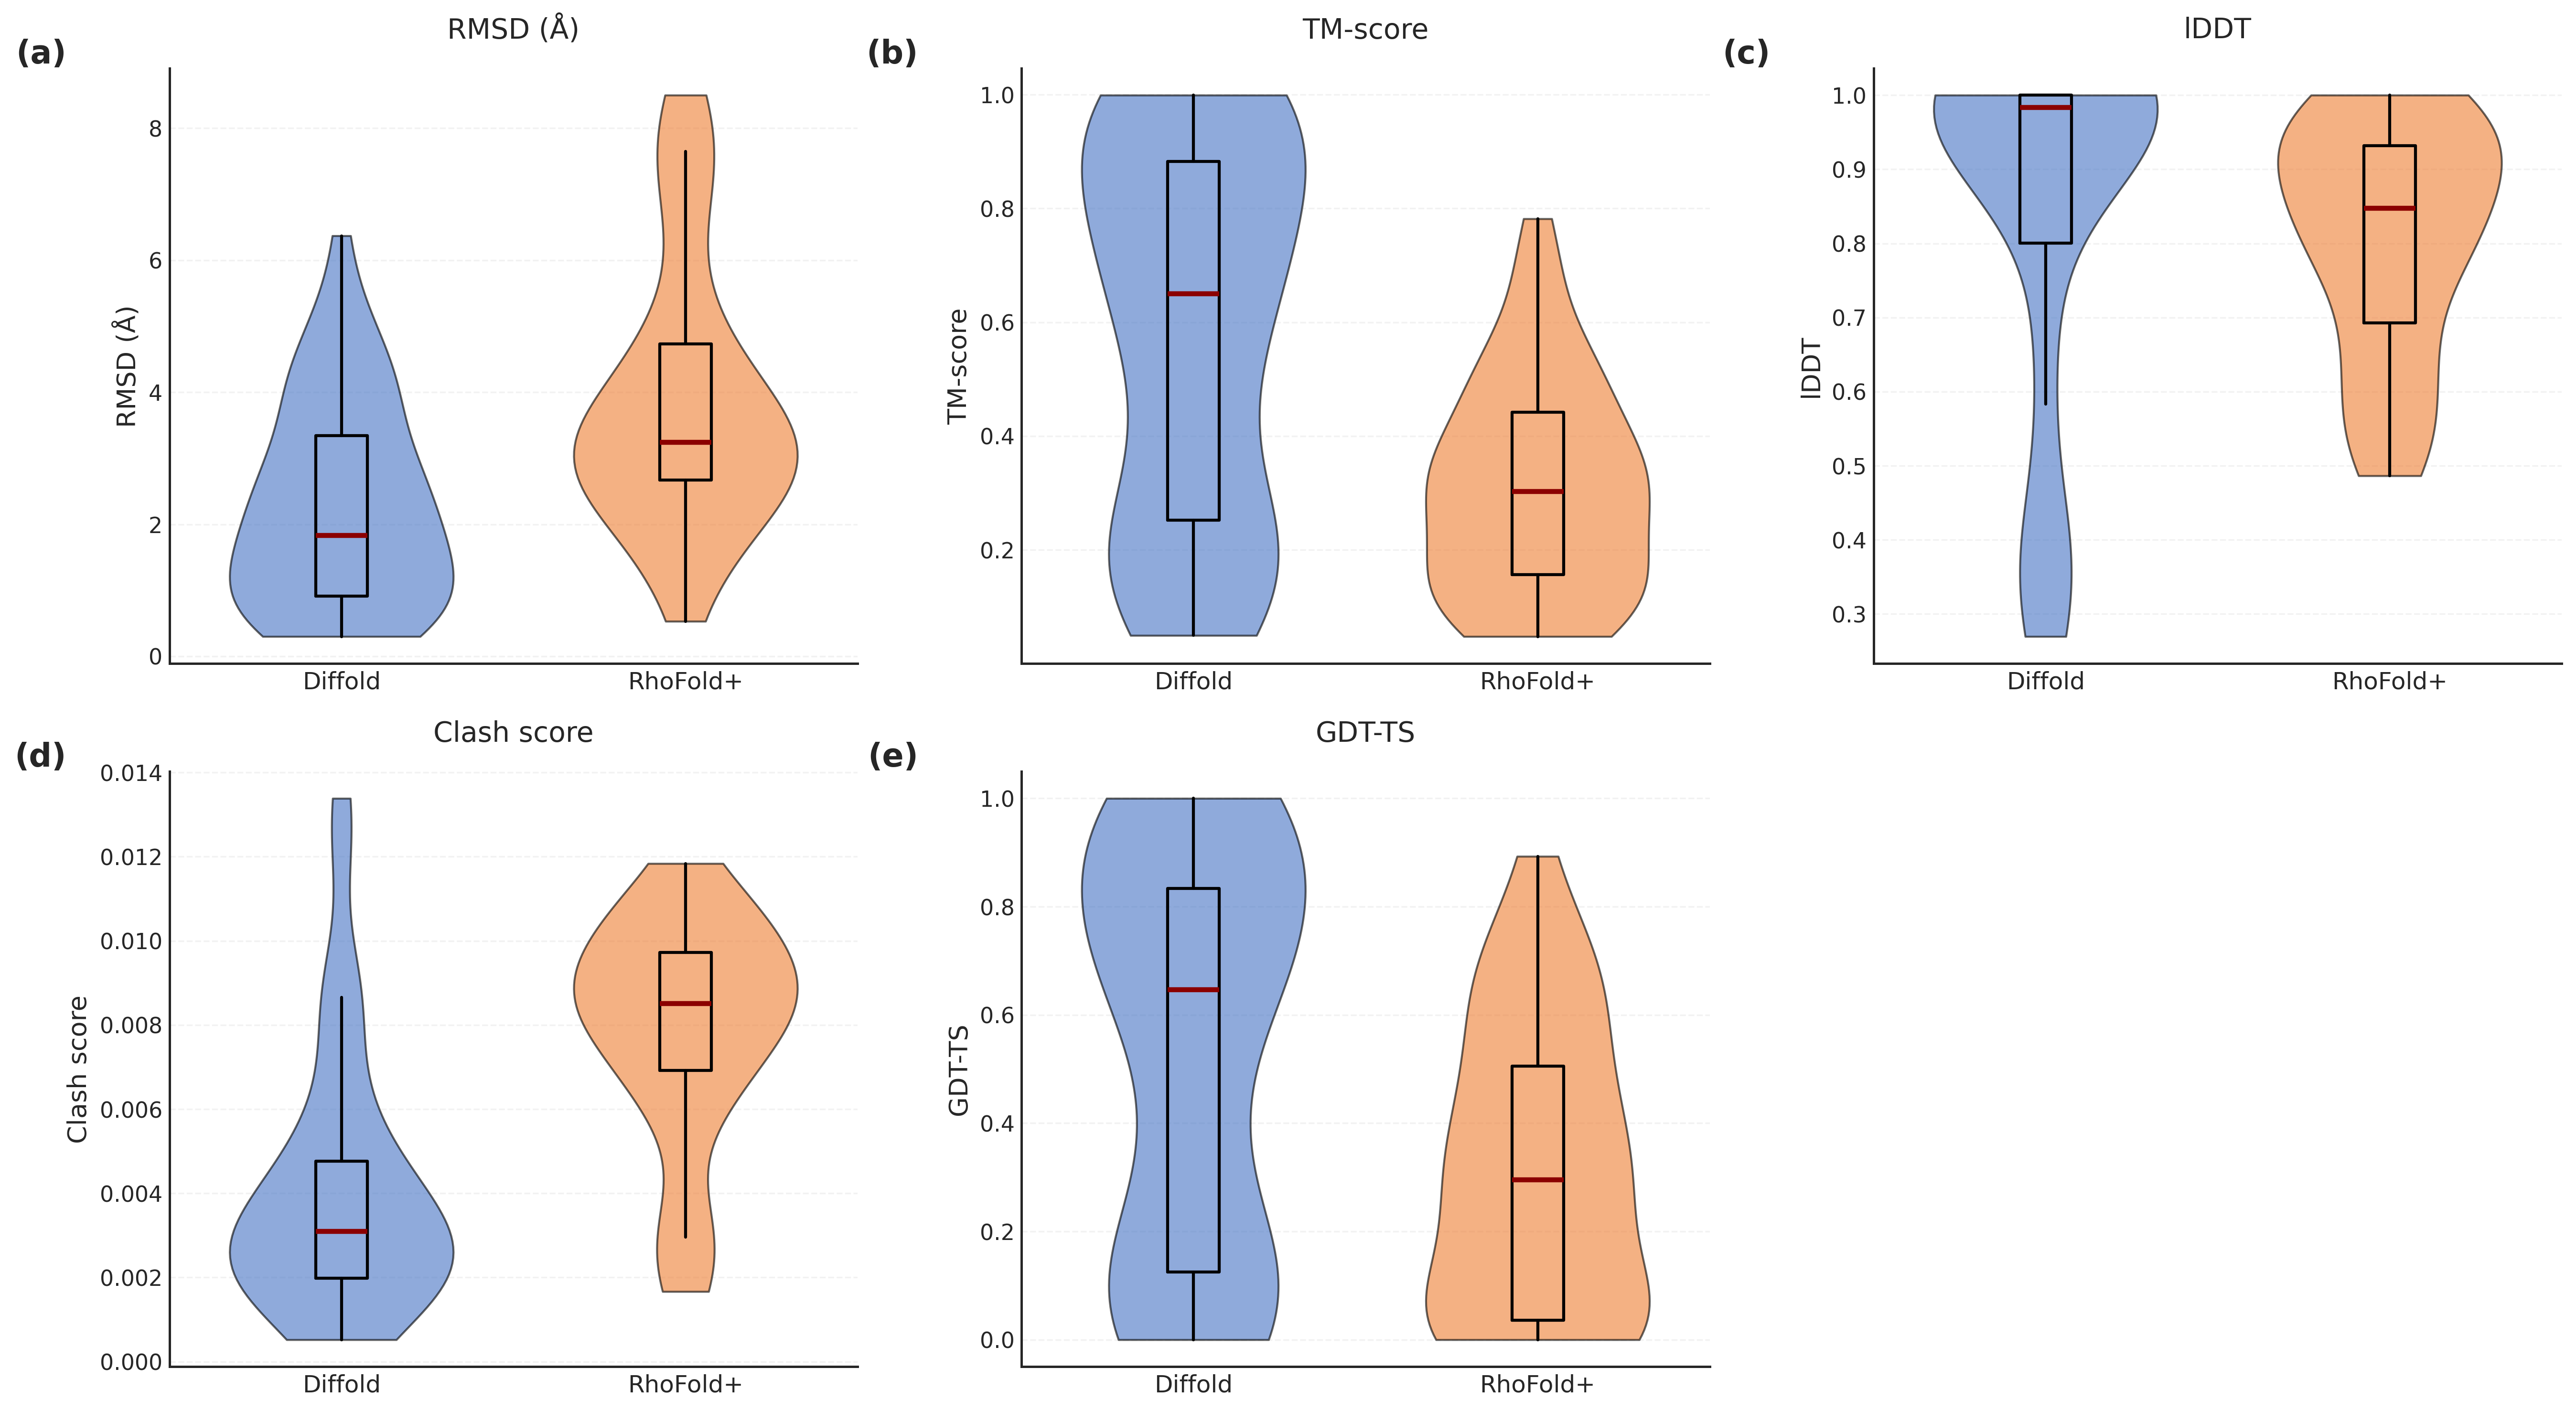
\includegraphics[width=1\linewidth]{img/Performance.png}
    \caption{Overall performance comparison of Diffold and RhoFold+ on the CASP16 and RNA-benchmark test set. Violin plots show metric distributions with boxplots indicating the median and interquartile range: (a) RMSD, (b) TM-score, (c) lDDT, (d) clash score, and (e) GDT-TS}
    \label{fig:performance}
\end{figure}

\begin{figure}
    \centering
    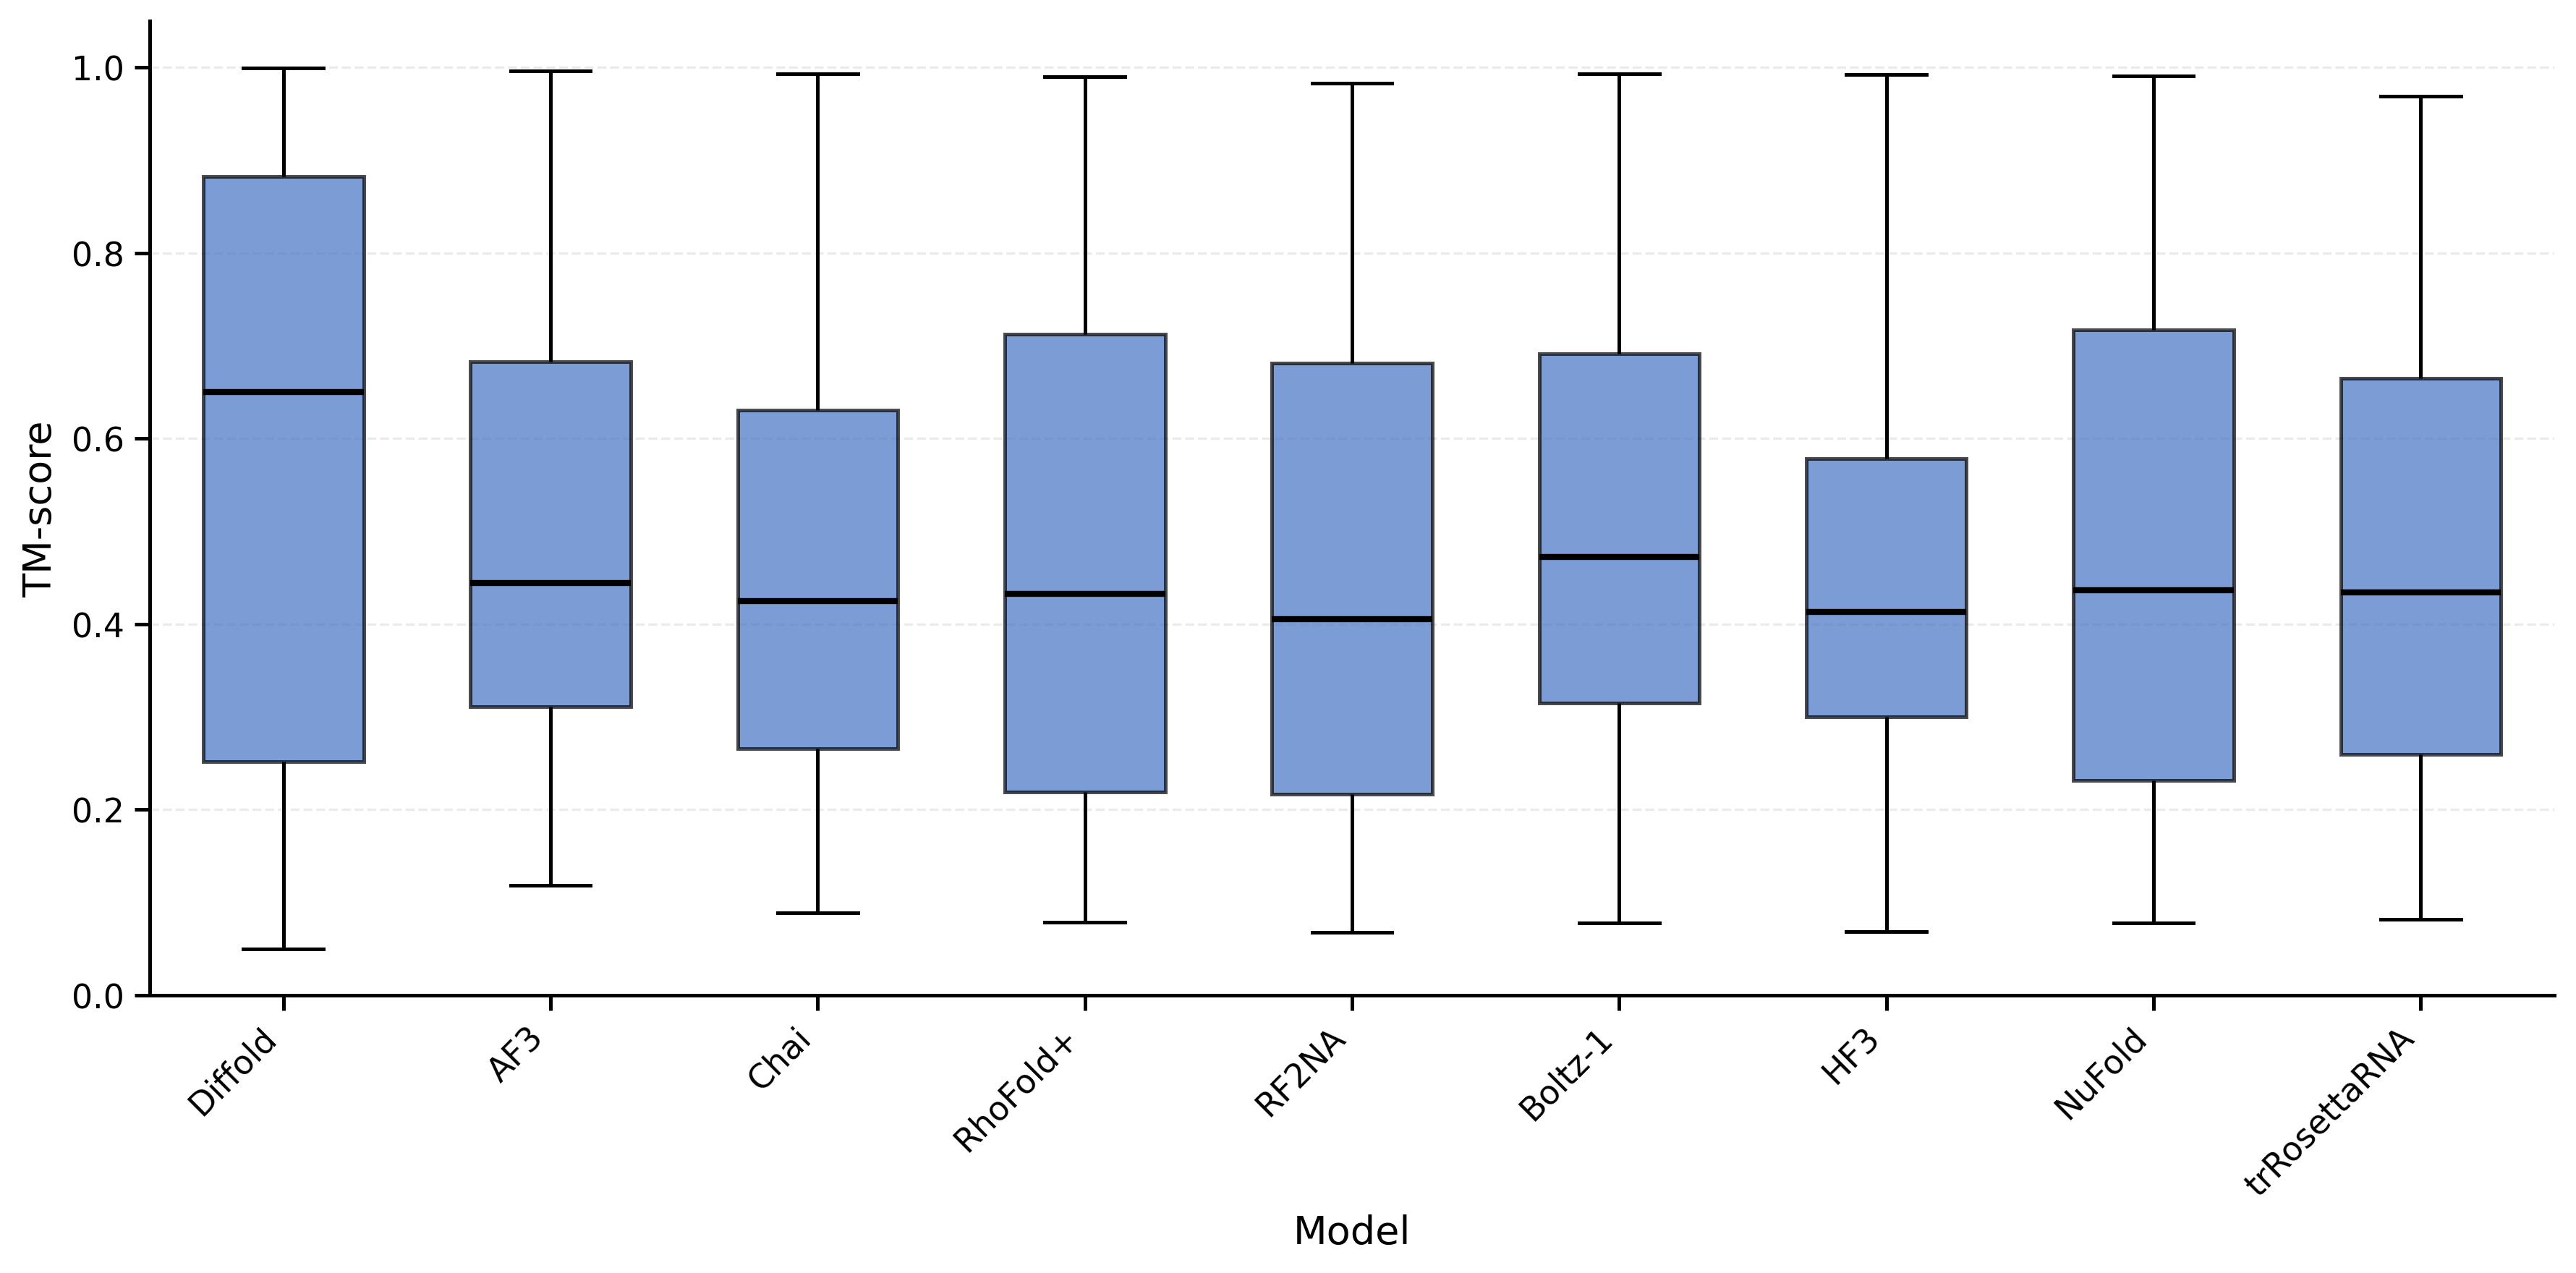
\includegraphics[width=1\linewidth]{img/Models_comparison.png}
    \caption{Cross-model comparison on RNA-Benchmark. TM-score distributions for Diffold and representative baselines}
    \label{fig:tmscore}
\end{figure}

\section{Performance Analysis}

\subsection{Sequence Length Analysis}

Across the combined CASP16 and RNA-benchmark test set, we further examined how prediction quality varies with sequence length (Fig. 4.3). As expected, RhoFold+ shows a clear length-dependent degradation: TM-score decreases with increasing length ($r=-0.440$, $p=7.7\times10^{-4}$), lDDT also decreases ($r=-0.391$, $p=3.1\times10^{-3}$), and GDT-TS exhibits an even stronger negative trend ($r=-0.573$, $p=4.9\times10^{-6}$), while RMSD increases sharply with length ($r=0.928$, $p=2.3\times10^{-24}$). In contrast, Diffold demonstrates markedly weaker length sensitivity for local and distance-based metrics, with near-zero correlations for RMSD ($r=0.011$, $p=0.94$) and lDDT ($r=0.021$, $p=0.88$), and only a mild, non-significant trend for GDT-TS ($r=0.126$, $p=0.35$). Notably, Diffold exhibits a positive correlation between TM-score and sequence length ($r=0.504$, $p=7.5\times10^{-5}$), which is counter to the commonly observed negative relationship in structure prediction. We attribute this phenomenon to a combination of data and model factors: first, Diffold was trained on RNAs with length limited to 16–256 nt, yet maintains stable accuracy on longer targets, suggesting favorable length generalization of the diffusion-based generator beyond the training regime; second, the distribution of test targets is uneven across lengths, and the subset of long RNAs may be enriched for more regular, helix-dominant folds that are comparatively easier to capture at the global topology level, thereby yielding higher TM-scores; third, shorter RNAs can contain highly flexible motifs and sparse evolutionary signal, and TM-score can be more sensitive to small absolute coordinate errors on short chains, which may collectively depress TM-score in the short-length regime. Therefore, while the positive TM-score–length trend should be interpreted with caution given potential composition bias in the test set, the overall pattern supports the conclusion that Diffold is substantially less affected by increasing sequence length than RhoFold+ and generalizes well to longer RNAs despite the absence of above 256 nt examples during training.

\begin{figure}
    \centering
    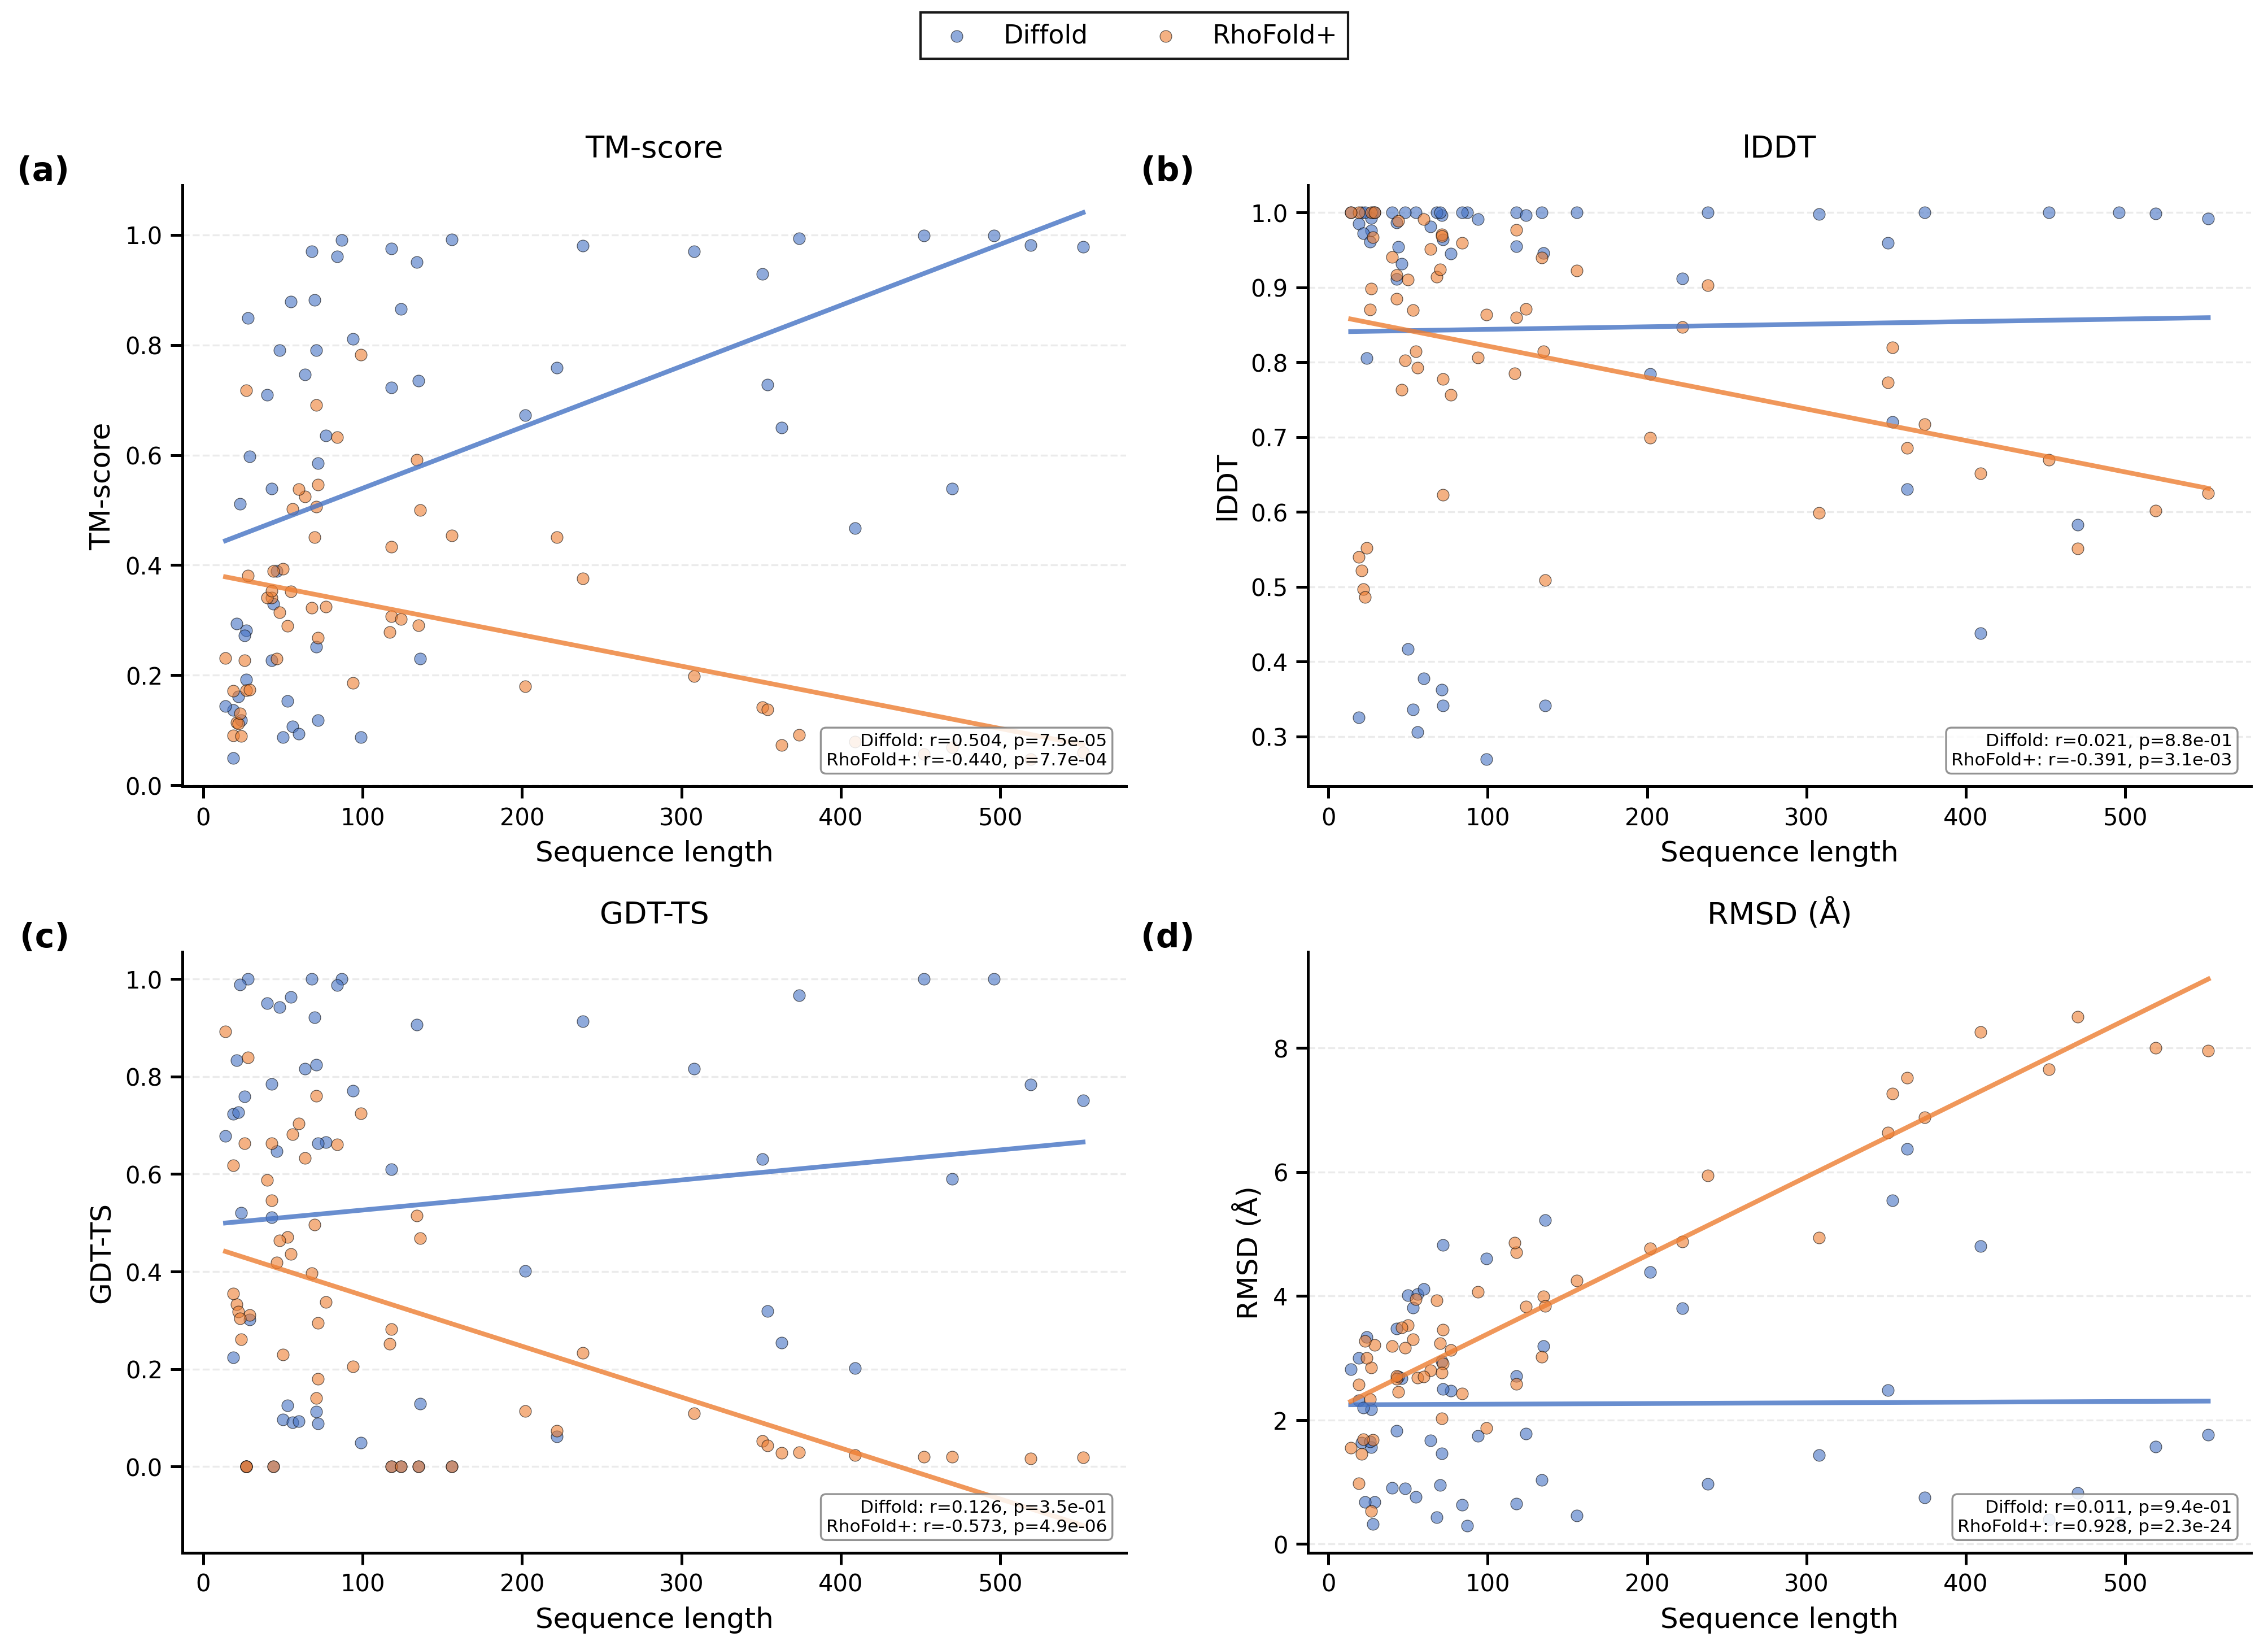
\includegraphics[width=1\linewidth]{img/Length_analysis.png}
    \caption{Relationship between sequence length and prediction metrics. Scatter plots report TM-score, lDDT, GDT-TS, and RMSD versus sequence length for Diffold and RhoFold+, with linear regression trends and correlation statistics.}
    \label{fig:length vs performance}
\end{figure}

\subsection{Dataset Dependence Analysis}

\begin{figure}
    \centering
    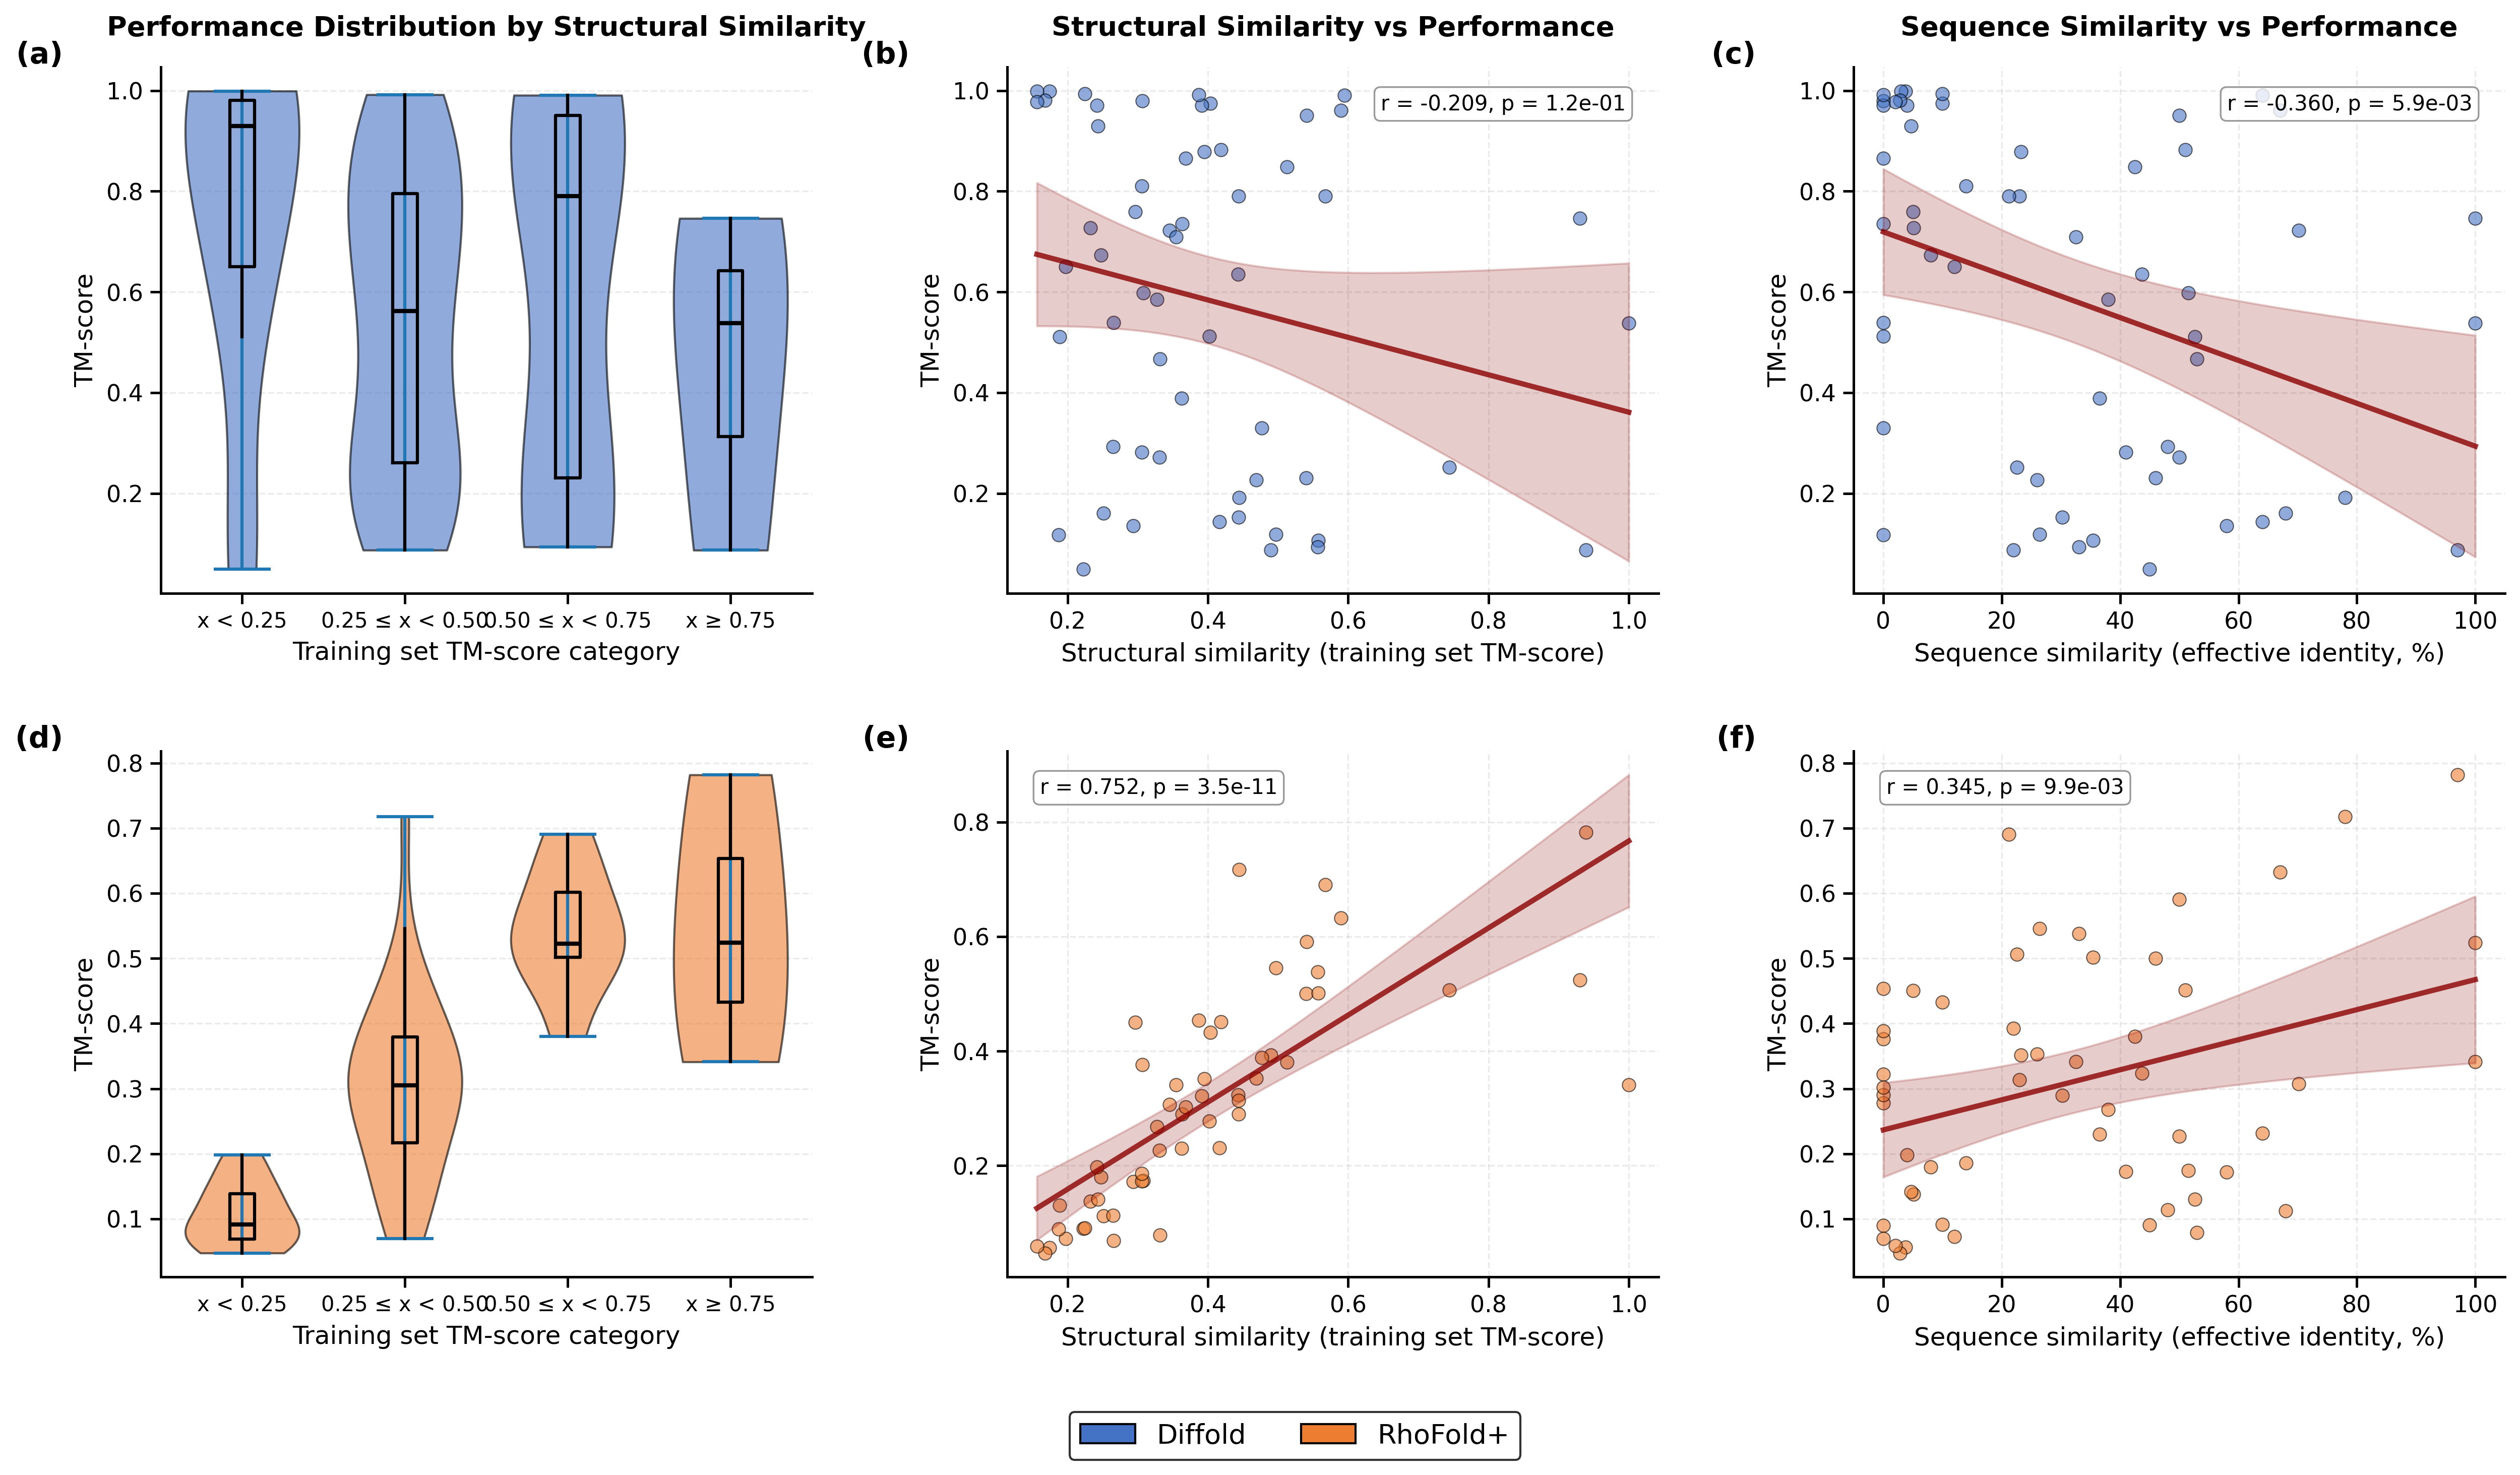
\includegraphics[width=1\linewidth]{img/new_dependence_analysis.png}
    \caption{Performance versus train–test similarity. (a–c) Diffold and (d–f) RhoFold+ on the test set. Train–test structural similarity is defined as the maximum TM-score of each test target to any training structure, and sequence similarity as the maximum BLAST effective identity to any training sequence. Violin plots show performance stratified by bins; scatter plots show per-target performance versus similarity (Pearson $r$, $p$ shown).}
    \label{fig:dependence}
\end{figure}

To assess data independence and potential memorization effects, we analyzed train--test similarity at both the structural and sequence levels (Fig.~4.4). For each test target $T$, we quantified its nearest-neighbor structural proximity to the training set as $\mathrm{Indep}_{\mathrm{struct}}(T)$, defined by the maximum TM-score between the native structure of $T$ and any native training structure, and examined how prediction accuracy varies with this similarity. Diffold shows no significant dependence on training-set structural proximity, with a weak and non-significant correlation ($r=-0.209$, $p=1.2\times10^{-1}$; Fig.~4.4b) and broadly comparable TM-score distributions across structural similarity bins (Fig.~4.4a). In contrast, RhoFold+ exhibits a strong positive association between performance and training-set structural similarity ($r=0.752$, $p=3.5\times10^{-11}$; Fig.~4.4e), and its TM-score increases substantially as the closest training neighbor becomes more similar. This pattern suggests that RhoFold+ benefits more from the presence of structurally similar examples in the training set, whereas Diffold is less tied to nearby structural neighbors.

We further repeated the analysis using the nearest-neighbor sequence proximity $\mathrm{Indep}_{\mathrm{seq}}(T)$, computed as the maximum BLAST effective identity between each test sequence and any training sequence. Notably, Diffold exhibits a negative association between performance and sequence similarity ($r=-0.360$, $p=5.9\times10^{-3}$; Fig.~4.4c), while RhoFold+ shows a modest but significant positive association ($r=0.345$, $p=9.9\times10^{-3}$; Fig.~4.4f). A likely explanation for this apparent anomaly is that, for RNA, sequence proximity is an imperfect surrogate for structural proximity: homologous RNAs may share conserved motifs yet differ in global fold, domain organization, or long-range/pseudoknotted interactions, so targets with high $\mathrm{Indep}_{\mathrm{seq}}$ can remain structurally novel and difficult. Moreover, BLAST is local-alignment based; high effective identity can still be driven by a conserved segment within a longer or multi-domain construct, inflating $\mathrm{Indep}_{\mathrm{seq}}$ without implying an easier whole-structure prediction problem. A third possibility is conflicting supervision among near-homologs in the training set (e.g. different constructs, bound states, or alternative conformations), which yields a multi-modal conditional distribution; a diffusion generator that models a broader ensemble may distribute probability mass across modes, reducing the likelihood of matching the single reference structure used for evaluation. Finally, $\mathrm{Indep}_{\mathrm{seq}}$ may correlate with confounders such as sequence length or structural complexity; if high-$\mathrm{Indep}_{\mathrm{seq}}$ targets are systematically harder, a negative correlation can emerge even in the absence of memorization. Taken together, the structural and sequence diagnostics consistently indicate that RhoFold+ benefits more from train-test proximity, whereas Diffold maintains competitive accuracy even when structurally distant from the training set, supporting stronger generalization and improved data independence under this evaluation protocol.


\section{Case Study}

\subsubsection{Case1: 8UYG}

For 8UYG, a 135-nt RNA target, we observed that directly generated all-atom coordinates occasionally violate covalent geometry along the RNA backbone, most notably the $\text{O3}'–\text{P}$ phosphodiester bonds, resulting in apparent chain breaks. Quantitatively, before relaxation, 75 $\text{O3}'–\text{P}$ bonds exceeded 2.0 $\text{\AA}$ in length, whereas after AMBER-based relaxation this number decreased to 1, indicating that force-field energy minimization effectively repairs local bond-length pathologies while preserving the overall fold. This case supports the use of AMBER relax as a practical post-processing step to improve the chemical completeness and physical plausibility of diffusion-generated RNA structures, especially when bond-length constraints are not explicitly enforced during generation.


\begin{figure}[H]
    \centering
    % ----- image 1 -----
    \begin{minipage}{0.48\linewidth}
        \centering
        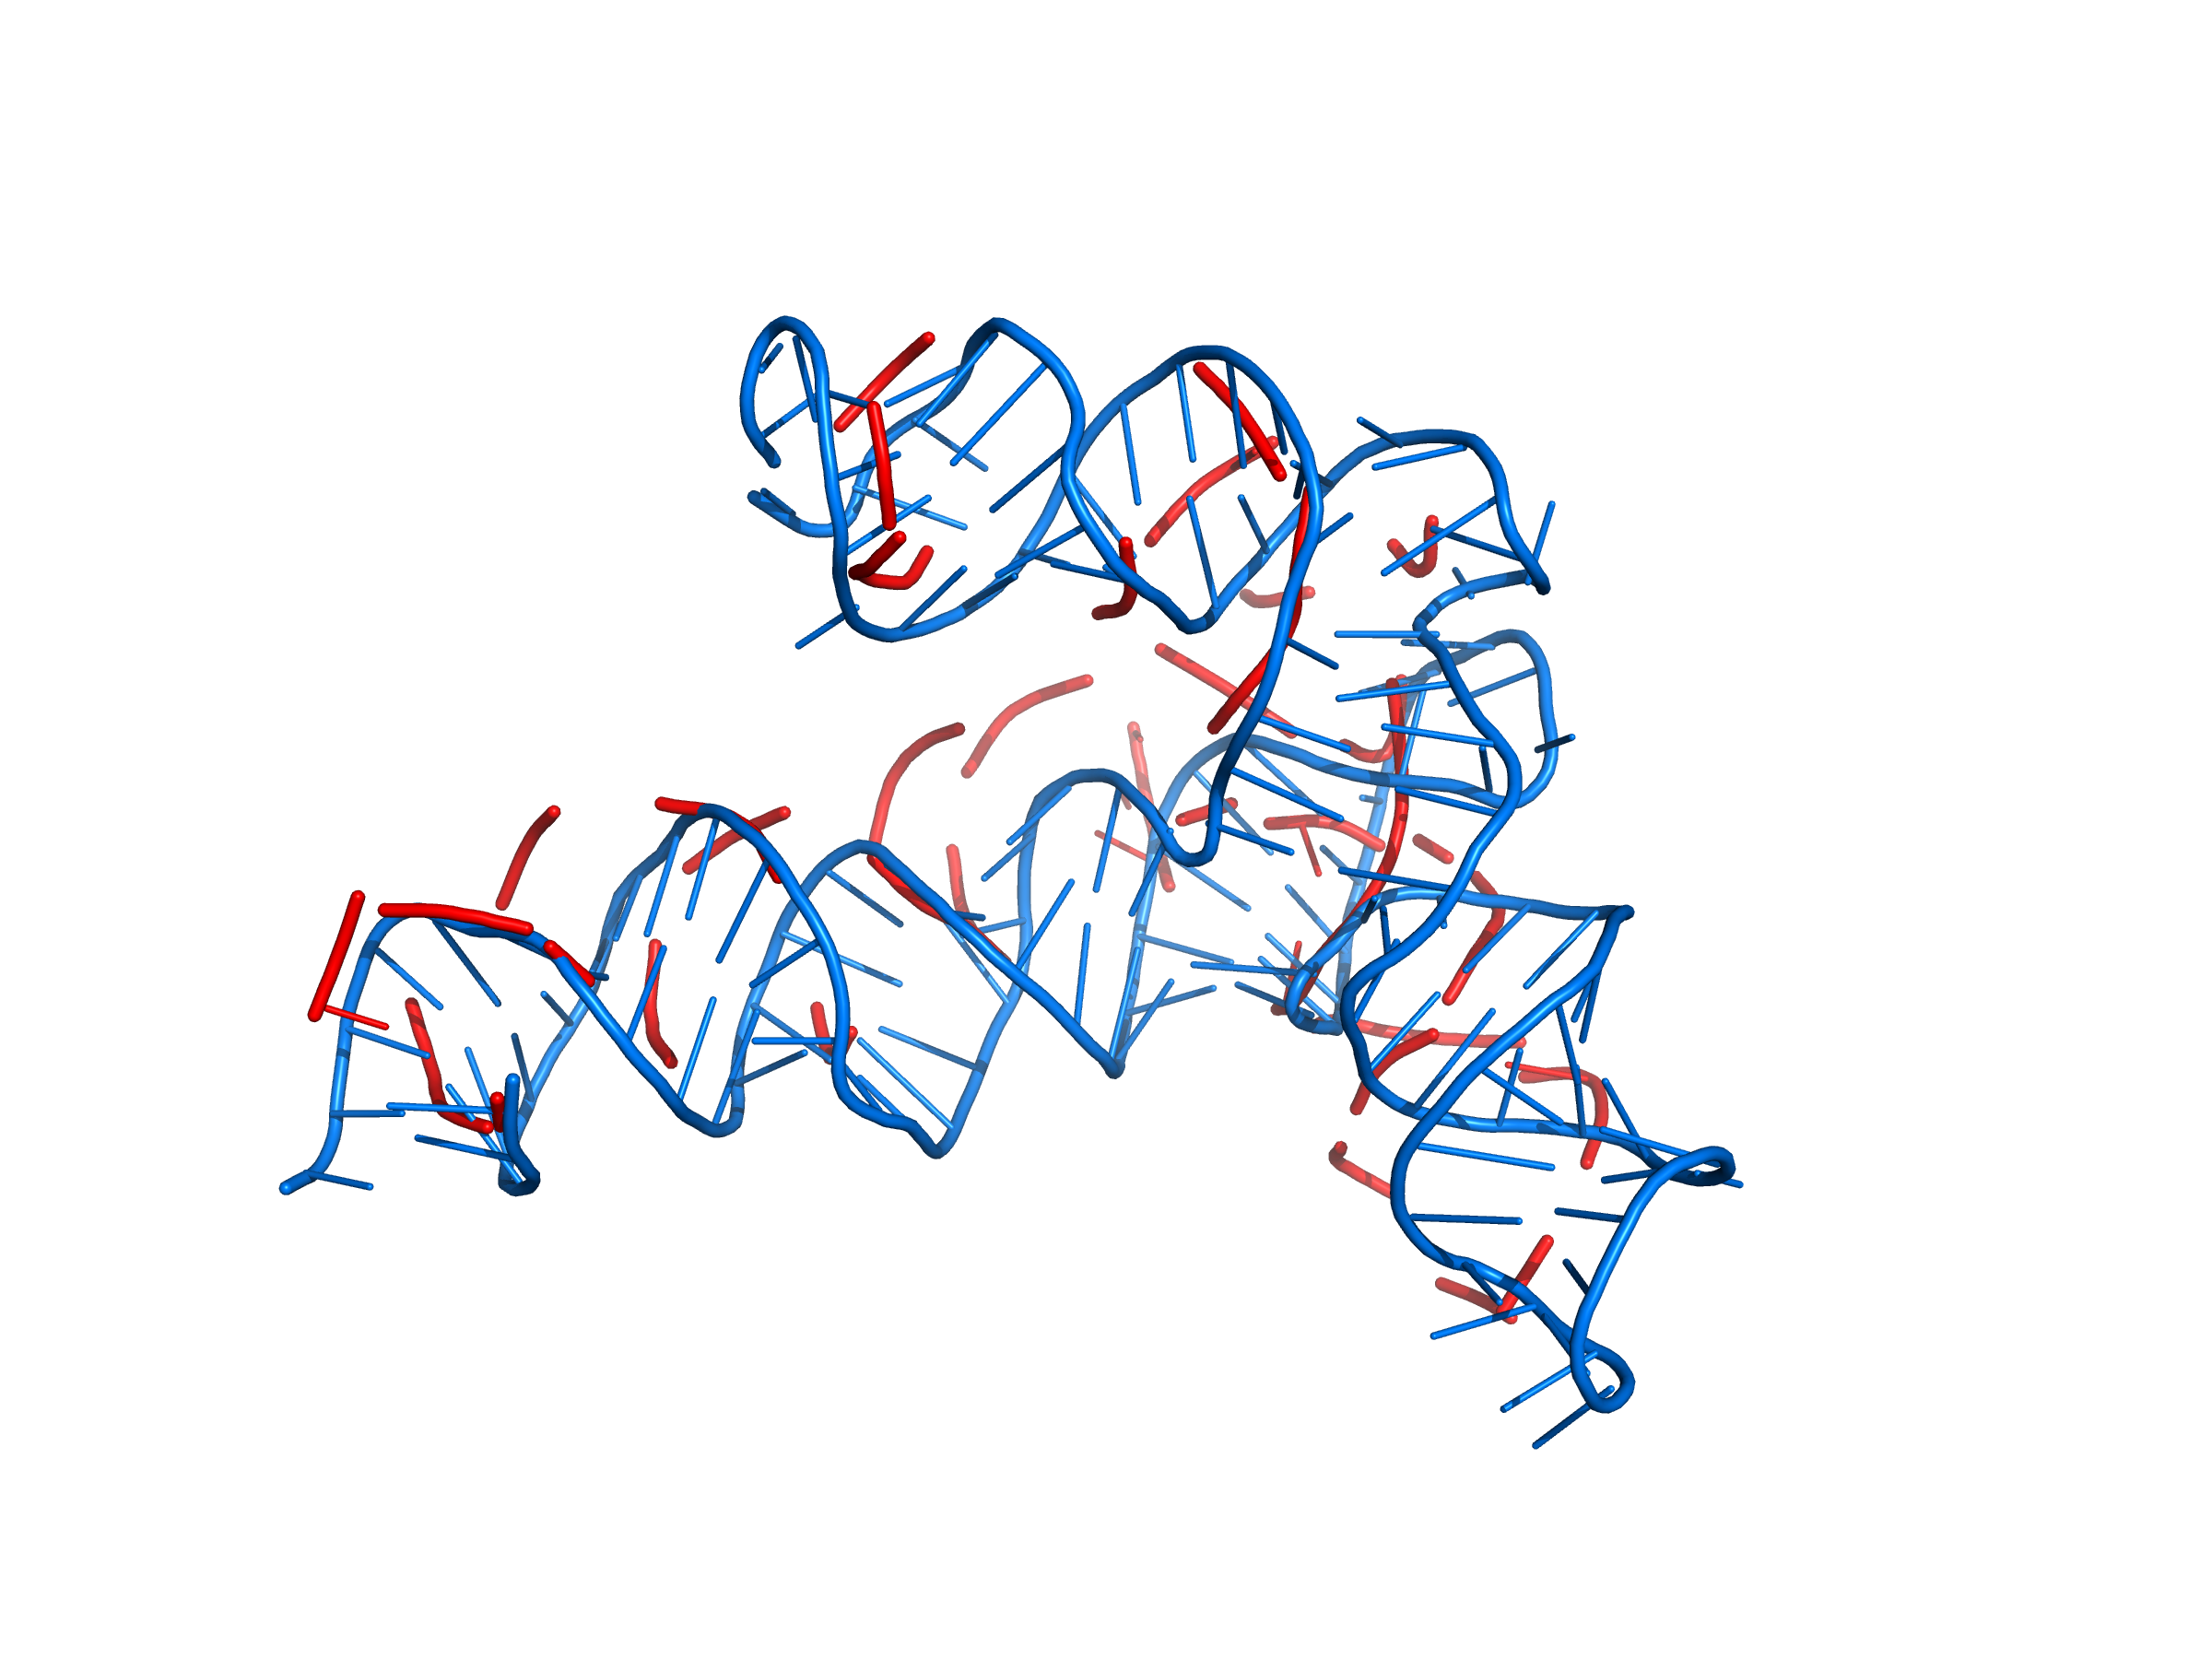
\includegraphics[width=\linewidth]{img/8uyg_pred_relaxed.png}
        \par (a)
    \end{minipage}
    \hfill
    % ----- image 2 -----
    \begin{minipage}{0.48\linewidth}
        \centering
        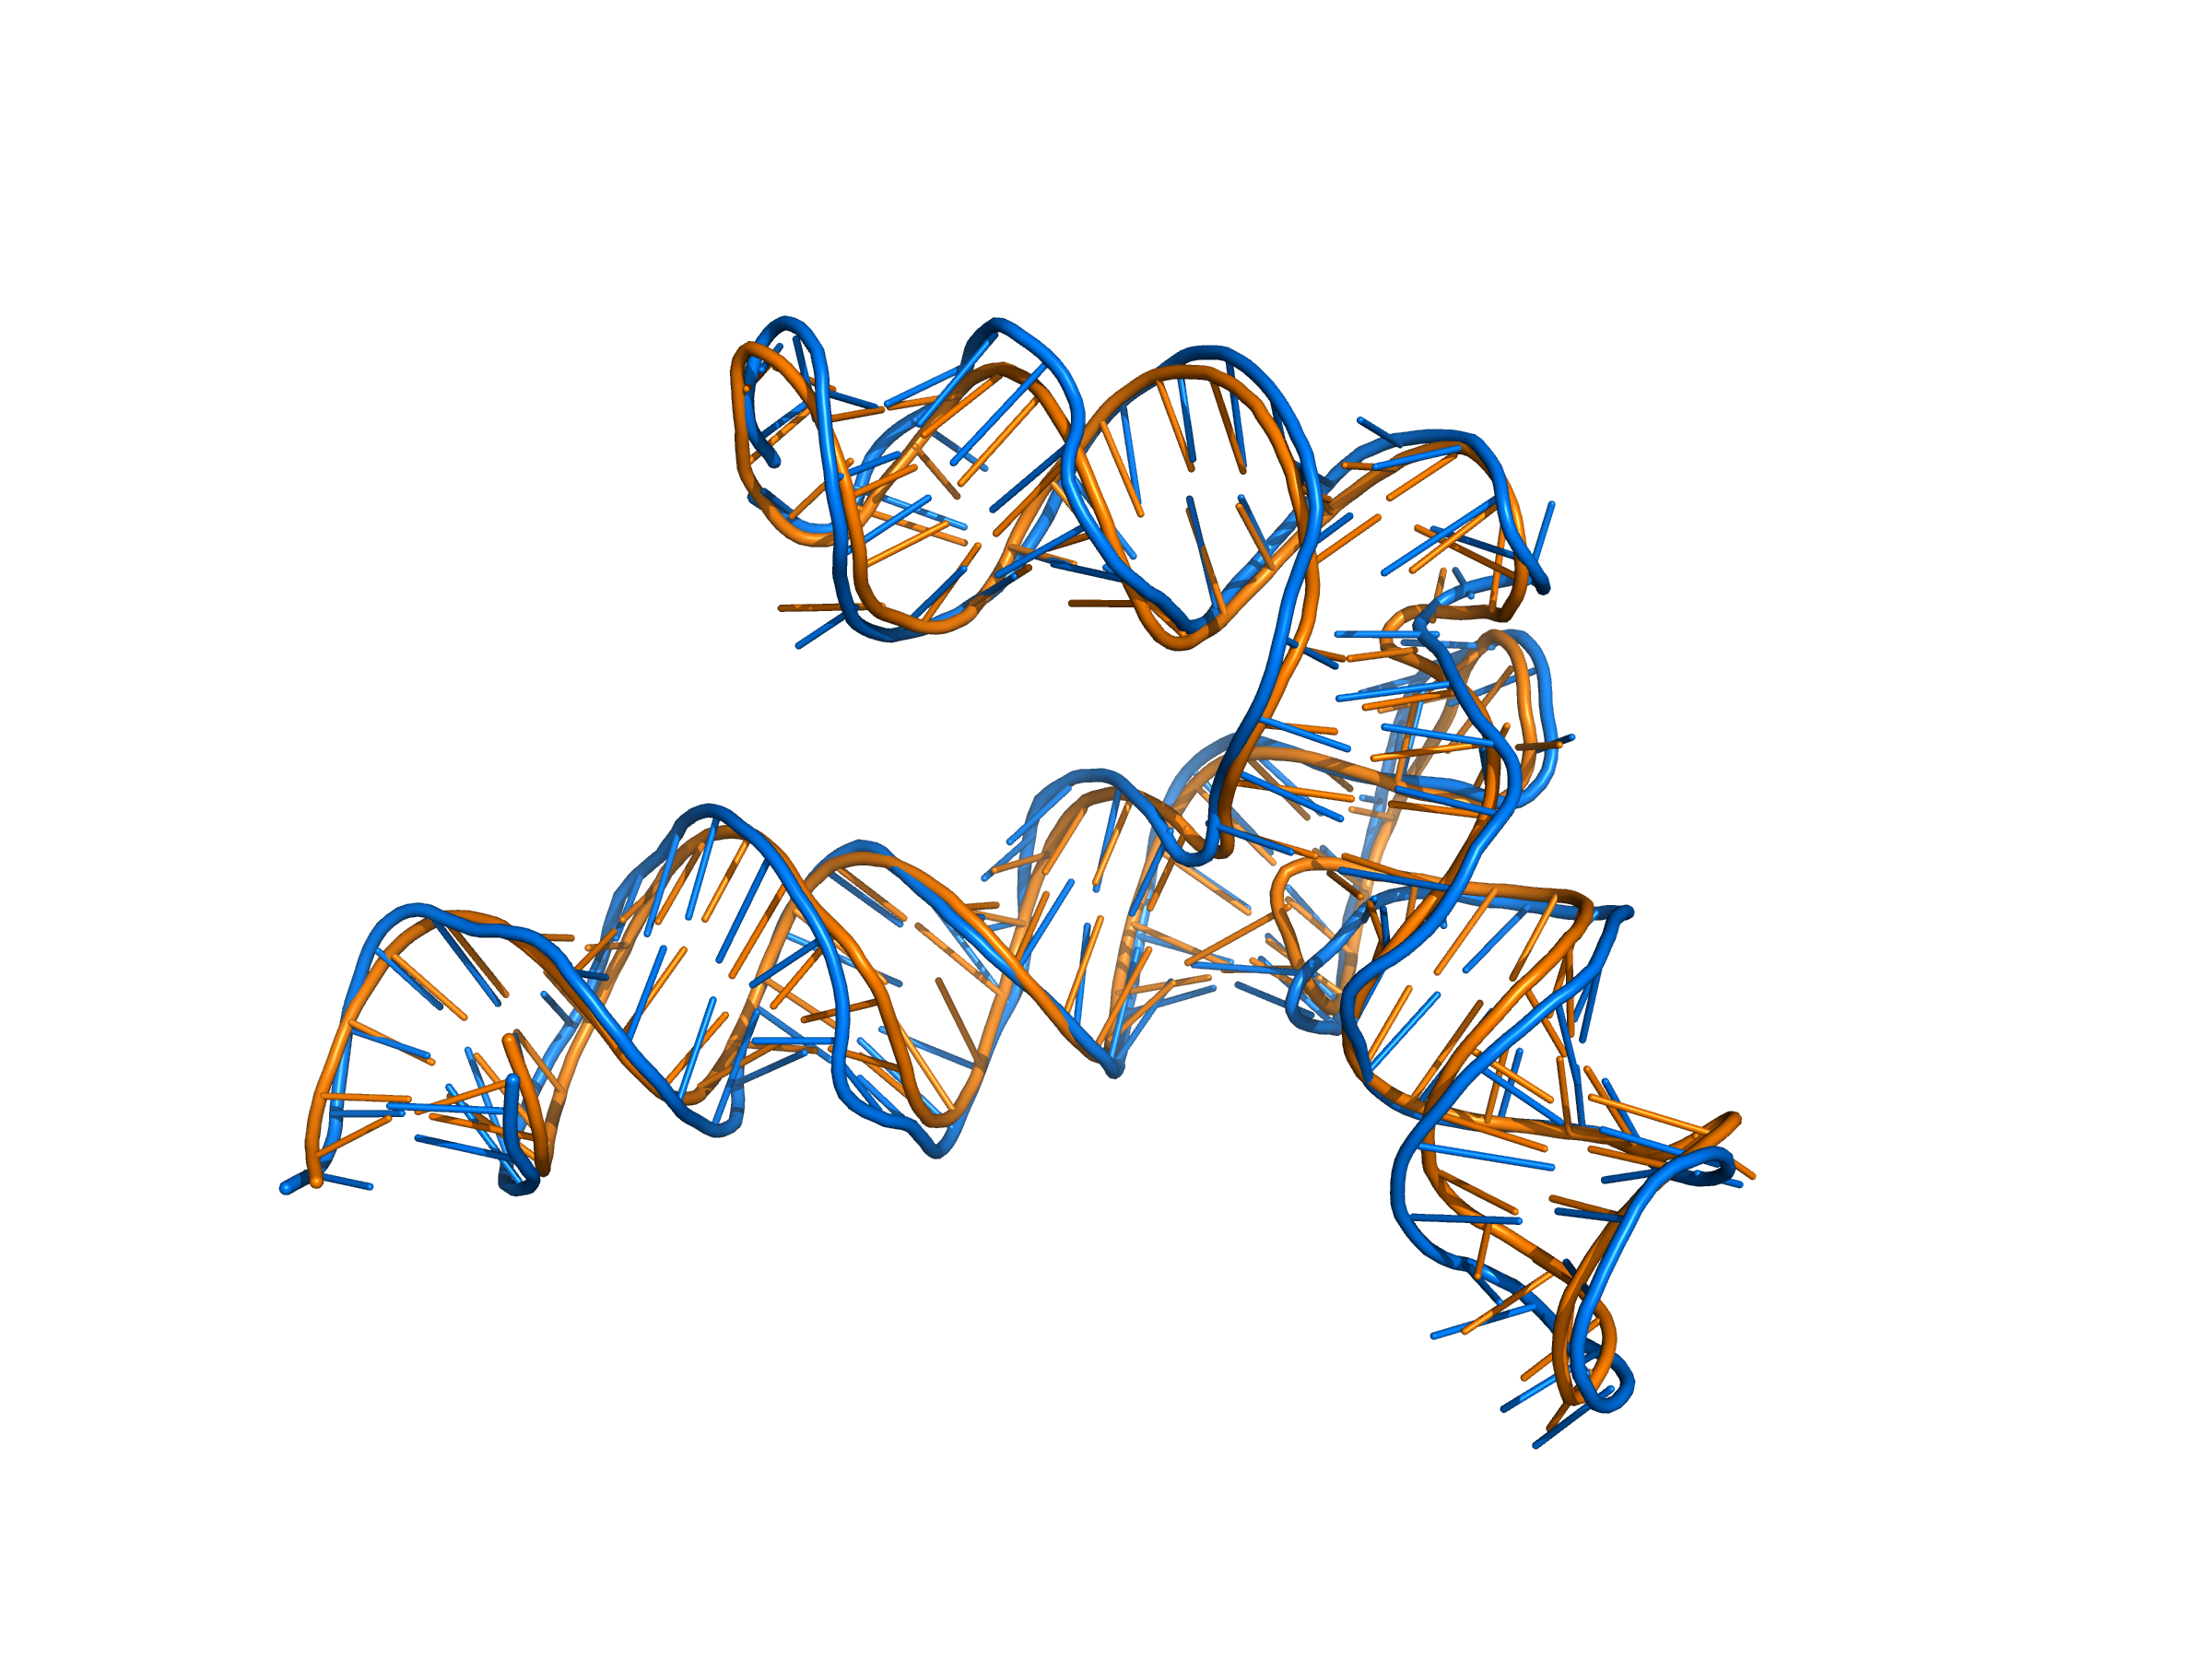
\includegraphics[width=\linewidth]{img/8uyg_pred_native.png}
        \par (b)
    \end{minipage}
    \caption{Structural alignment for PDB 8UYG before and after relaxation.
(a) Overlay of the unrelaxed prediction (red) with the native structure (blue).
(b) Overlay of the relaxed prediction (orange) with the native structure (blue).}
    \label{fig:8uyg}
\end{figure}

\begin{figure}[!htbp]
    \centering
    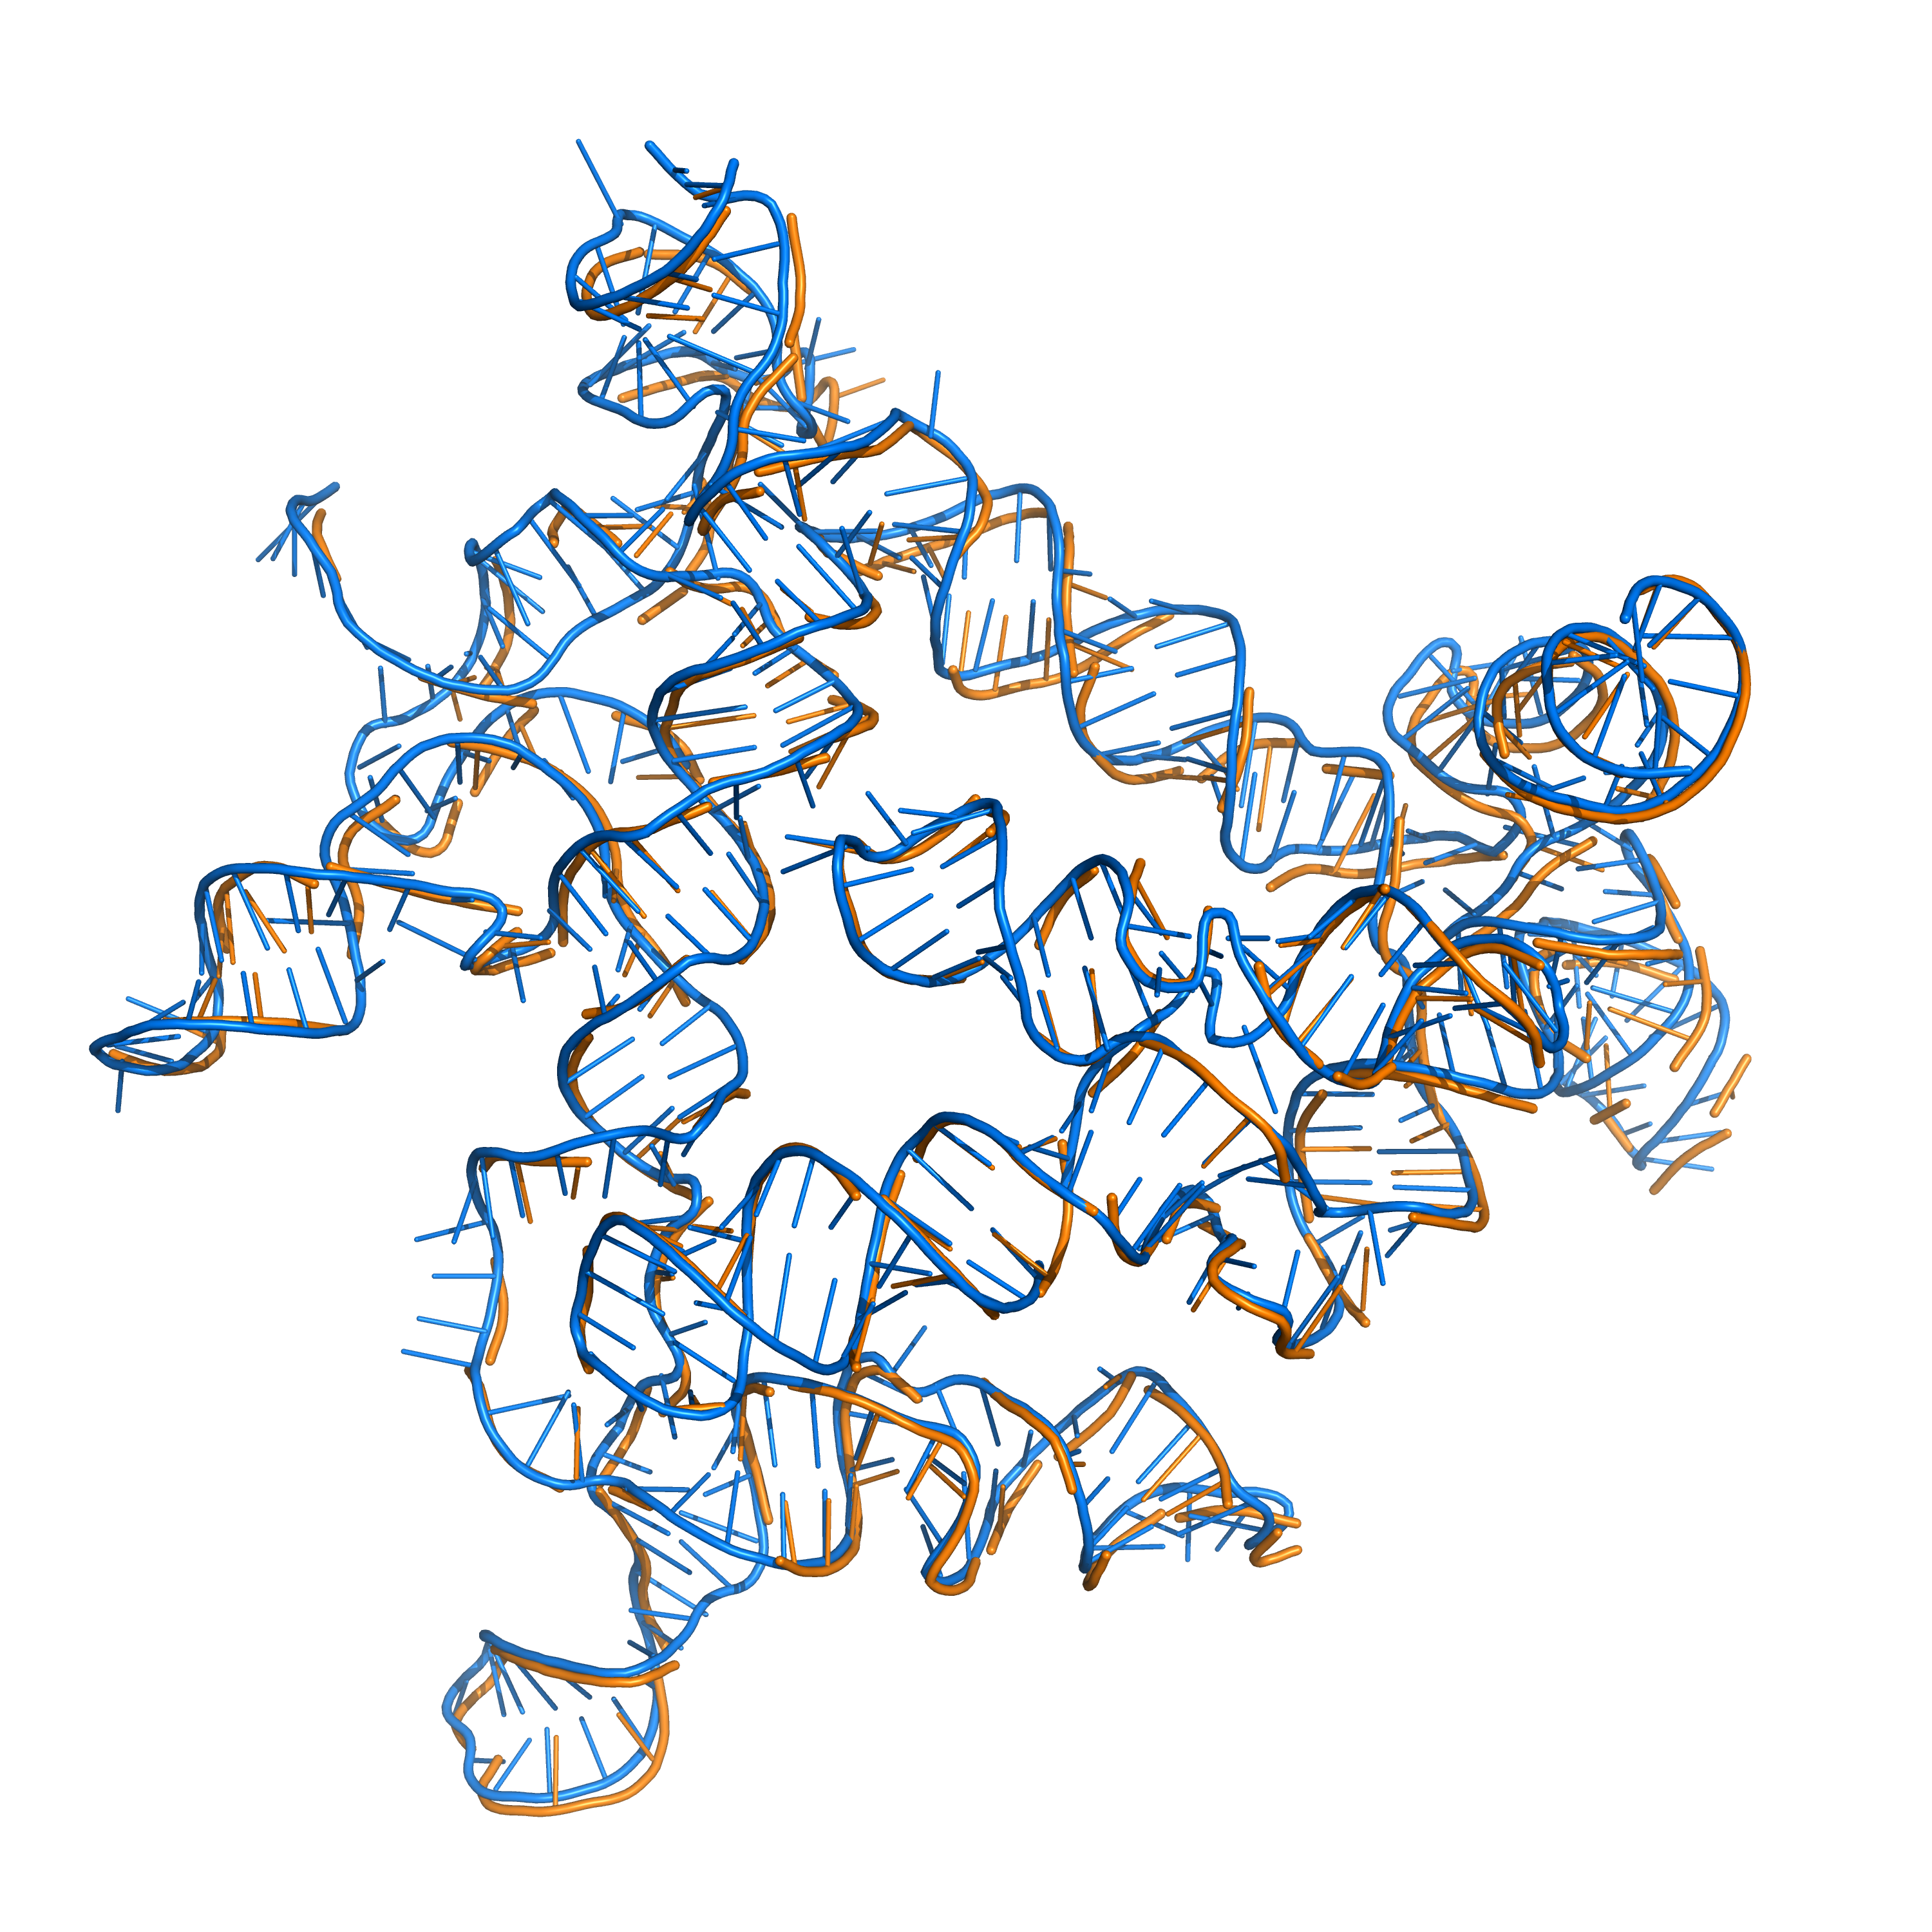
\includegraphics[width=0.5\linewidth]{img/R1283v2_pred_native.png}
    \caption{Structural alignment for R1283v2 (PDB 9J3R).
Overlay of the predicted structure (orange) with the native structure (blue).}
    \label{fig:placeholder}
\end{figure}

\subsubsection{Case2: 9J3R(R1283v2)}

The target R1283v2 corresponds to a long RNA (452 nt) represented by PDB 9J3R. On this target, RhoFold+ fails to recover the native topology, yielding a near-random alignment with TM-score 0.034, while Diffold achieves an almost native-quality reconstruction with TM-score 0.994. This striking gap is notable because the training regime constrains the RNA length to at most 256 nt, implying that Diffold can extrapolate beyond the training length regime and maintain long-range structural coherence at a scale of several hundred nucleotides.

At the same time, this case exposes a systematic geometry issue of Diffold: it tends to predict slightly elongated covalent distances along the backbone, most prominently the O3$'$\!--P linkage. For short RNAs, the subsequent relaxation step is highly effective at correcting these local bond-geometry deviations, restoring chain continuity without materially affecting the global fold. In contrast, for long targets such as R1283v2, the same bias accumulates over hundreds of nucleotides and manifests as widespread backbone discontinuities. Once many O3$'$\!--P distances exceed the bonding threshold, standard relax procedures provide only limited benefit: they can smooth local sterics and adjust nearby torsions, but they typically cannot globally re-establish covalent connectivity across numerous breaks without explicit bond-length restraints or dedicated connectivity-repair operations. Consequently, relaxation remains effective for short molecules but becomes nearly ineffective for long RNAs, even when the overall topology is largely correct.

Overall, R1283v2 highlights a separation between Diffold's strong global generalization and a length-amplified local backbone-geometry bias, suggesting that improving covalent-geometry constraints during generation or adding constraint-aware refinement will be important for robust long-RNA modeling.



\subsubsection{Case3: 7WIA}

In contrast, 7W1A represents a challenging failure case: although its nearest training-set structural neighbor reaches a maximum TM-score of 0.81, Diffold attains only TM-score 0.162, whereas RhoFold+ achieves 0.661 on the same target. This discrepancy indicates that training-set proximity alone is insufficient to guarantee successful generation, especially for compact, topology-sensitive RNAs.

A key observation is that Diffold's prediction for 7W1A exhibits severe backbone fragmentation (widespread chain discontinuities), such that the model produces locally plausible fragments but fails to assemble a single continuous fold. In this regime, standard relaxation offers limited benefit because it can smooth local sterics and adjust torsions, yet it cannot reliably re-establish covalent connectivity across many breaks without explicit bond-length restraints or dedicated connectivity-repair steps. Consequently, the evaluation against a single native reference yields a very low TM-score even if some local motifs are partially correct.

From a biological and biophysical perspective, 7W1A is a riboswitch target, and riboswitch RNAs are known to display pronounced conformational heterogeneity and environment-dependent folding: tertiary packing can depend on ligand binding, divalent ions, and specific stabilizing motifs. Under such conditions, a diffusion generator may either sample an alternative, physically reasonable conformer that scores poorly against one experimental snapshot, or become under-constrained when the evolutionary/MSA signal is weak and only a small number of long-range contacts determine the global topology. These factors can also explain why a high nearest-neighbor TM-score to the training set does not translate into high accuracy on this target.



\begin{figure}
    \centering
    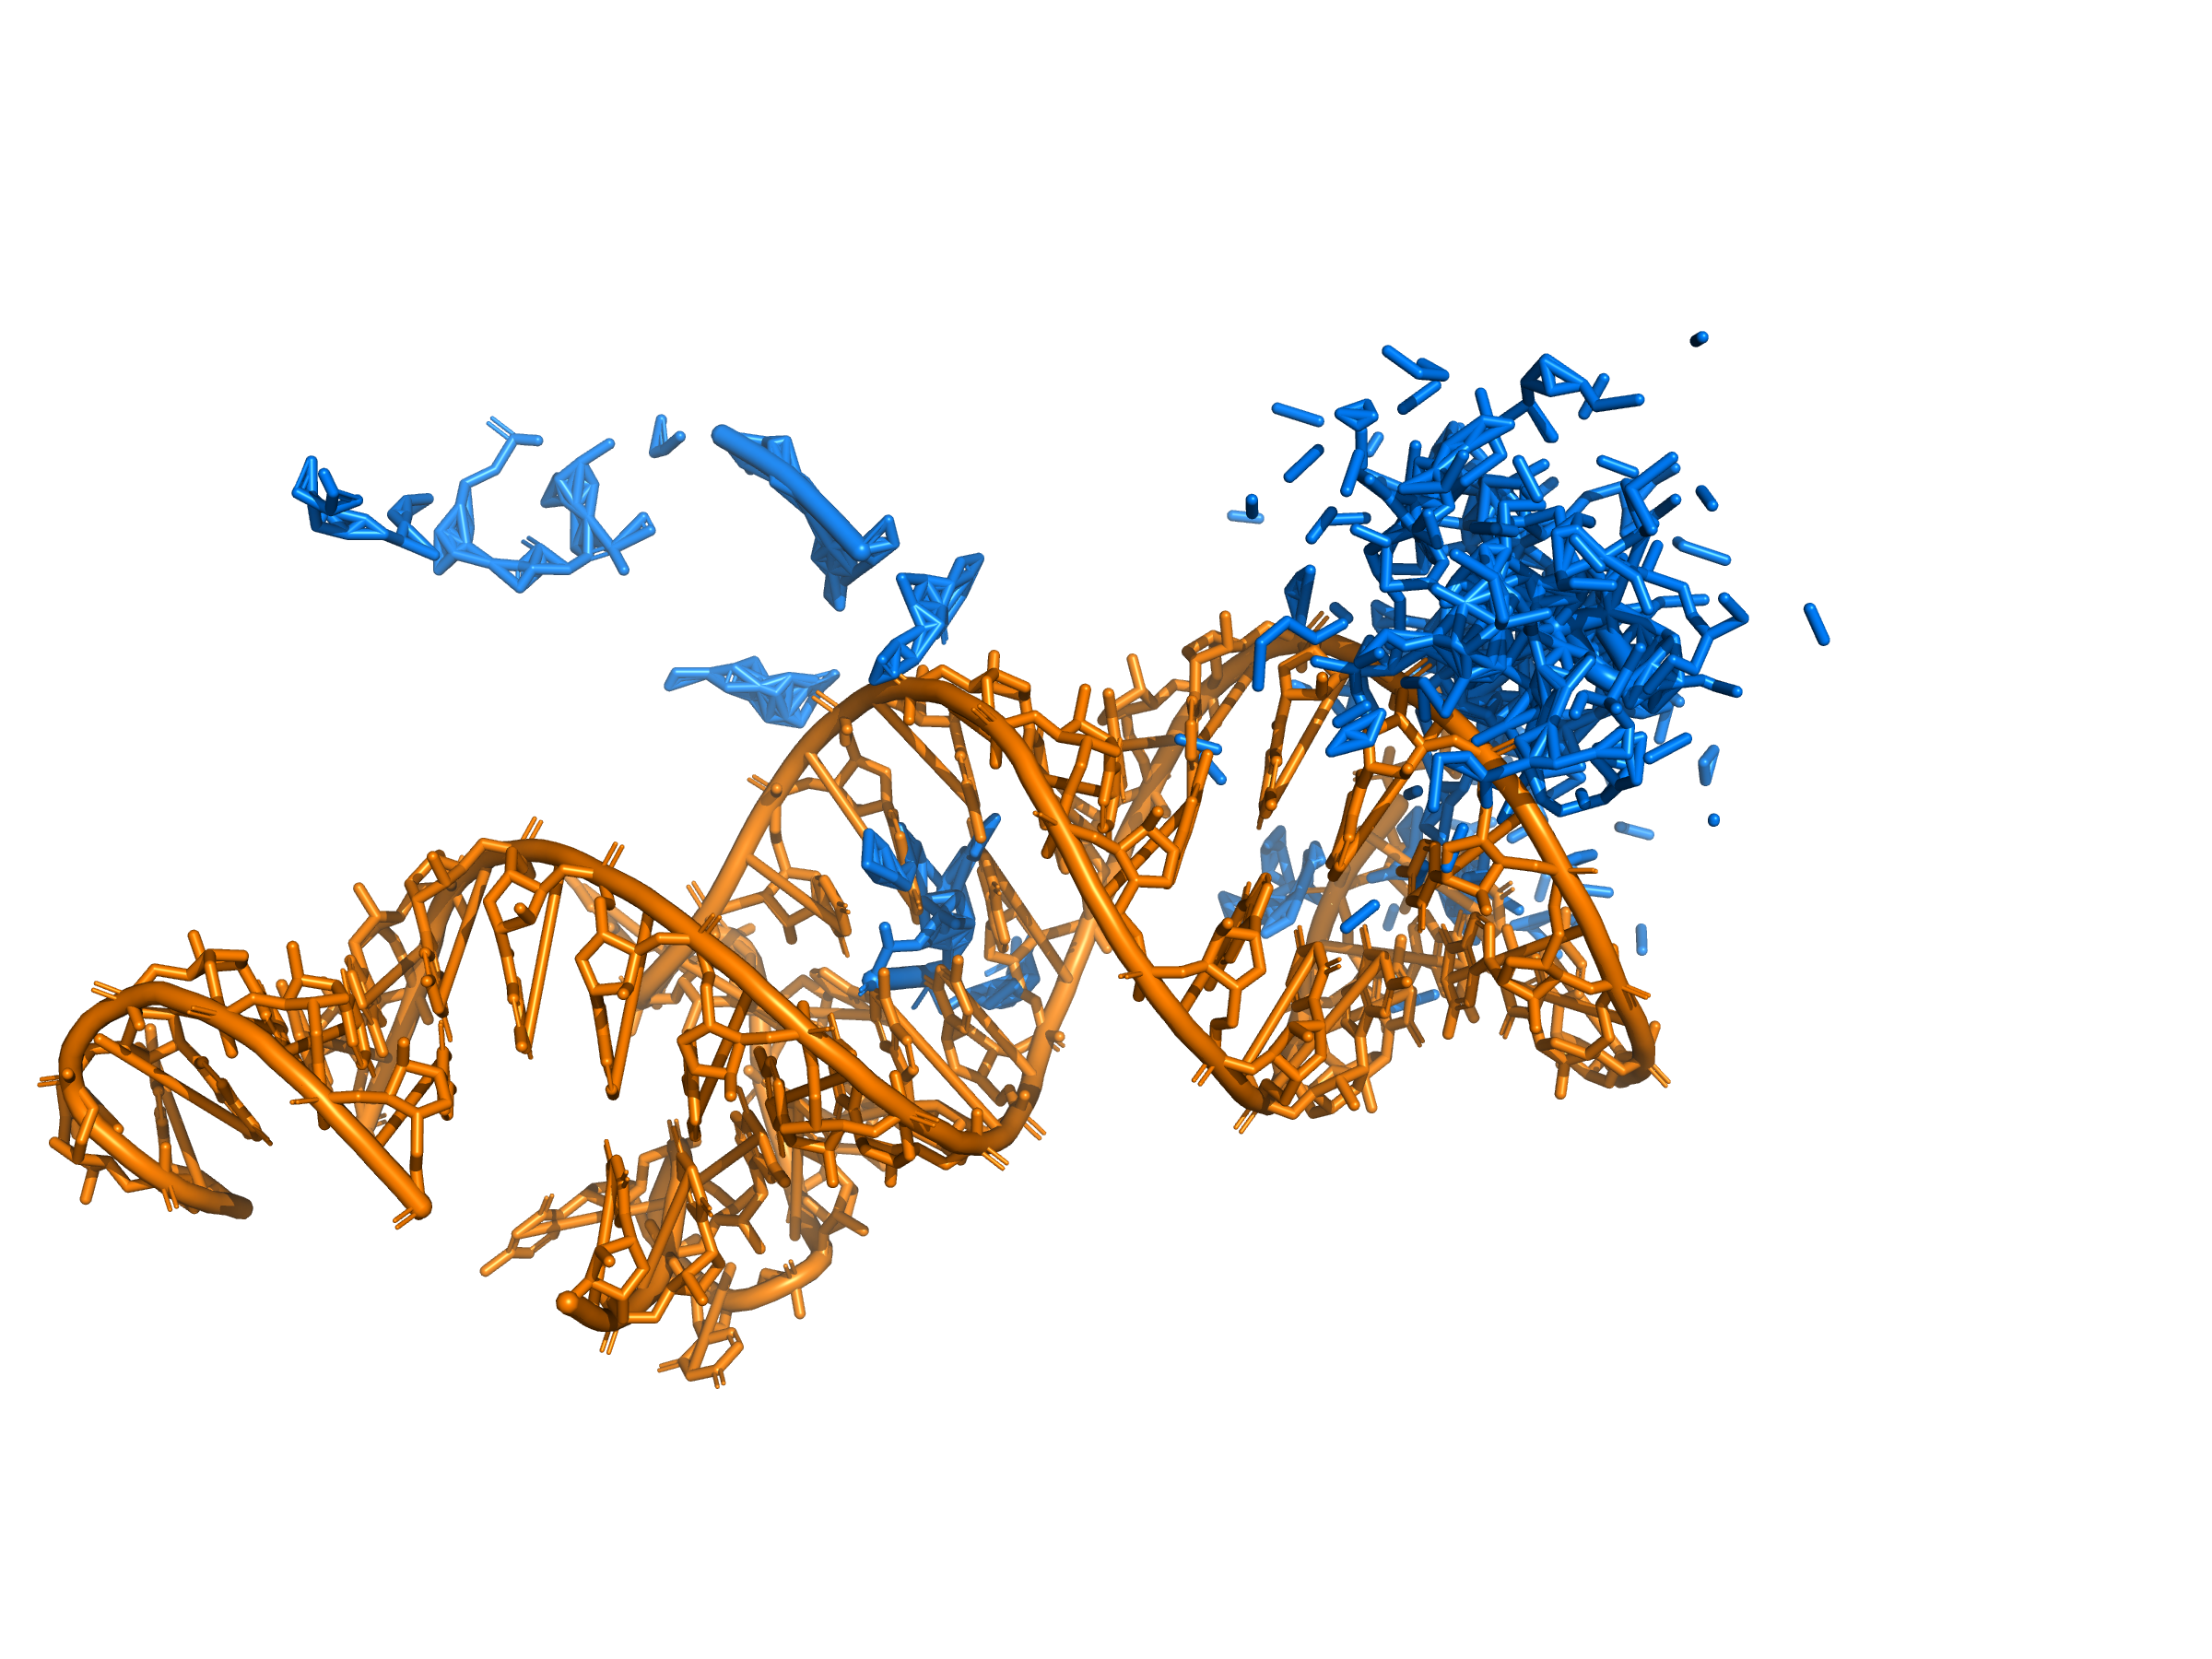
\includegraphics[width=1\linewidth]{img/7w1a_failure.png}
    \caption{Failure case on PDB 7W1A.
Predicted structure (orange) versus native structure (blue) visualized in a non-chain representation due to severe backbone discontinuities in the prediction.}
    \label{fig:placeholder}
\end{figure}
\chapter{Conclusion}

In this thesis, we introduced Diffold, a diffusion-based generative framework for RNA three-dimensional structure prediction that integrates (i) the geometric backbone and evolutionary representations of RhoFold+, (ii) structural priors from the large-scale RNA language model RNA-FM, and (iii) an Elucidated Diffusion Model (EDM) formulation for continuous-noise coordinate generation. By directly modeling all-atom coordinates through an iterative denoising process conditioned on residue- and atom-level features, Diffold aims to improve not only global fold recovery but also local geometric consistency and physical plausibility.

Comprehensive evaluation on the combined CASP16 and RNA-benchmark test set demonstrates that Diffold consistently surpasses the strong baseline RhoFold+ across all major accuracy and geometry metrics. Specifically, Diffold reduces RMSD from $3.85 \pm 1.96$ $\text{\AA}$ to $2.29 \pm 1.53$ $\text{\AA}$ (−40.5\%) and improves TM-score from $0.309 \pm 0.185$ to $0.585 \pm 0.328$ (+89.3\%), indicating substantially better global fold reconstruction. Consistently, GDT-TS increases from $0.313 \pm 0.262$ to $0.537 \pm 0.365$ (+71.5\%), further supporting improved backbone-level agreement with native structures. For local structural fidelity, Diffold achieves a higher lDDT ($0.845 \pm 0.247$ vs. $0.806 \pm 0.155$, +4.9\%), suggesting improved local geometric consistency on many targets. Importantly, Diffold also yields a markedly lower clash score ($0.0041 \pm 0.0030$ vs. $0.0079 \pm 0.0026$, −48.1\%), reflecting fewer severe steric conflicts and overall better physical plausibility of the generated all-atom conformations. When placed in a broader context using TM-score distributions across representative baselines, Diffold exhibits the highest median TM-score and remains competitive in spread, highlighting the advantage of diffusion-based generation under this evaluation setting.

Beyond aggregate accuracy, Diffold shows improved data independence under a training–test similarity diagnostic based on structural TM-score. Using the maximum TM-score between each test target and all training structures as a proxy for the closest training neighbor, Diffold exhibits only weak and non-significant dependence between test performance and training-set similarity $r = −0.209, p = (1.2\times10^{-1})$, whereas RhoFold+ shows a strong positive correlation $r = 0.752, p = 3.5\times10^{-11}$. This contrast suggests that Diffold’s diffusion generator is less reliant on template-like proximity to structurally similar training examples and can better generalize to structurally more distant targets under this protocol.

Finally, we demonstrated that a lightweight force-field-based post-processing step can effectively correct local covalent-geometry pathologies that may arise when generating coordinates directly in Cartesian space. In the 8UYG case (135 nt), the diffusion output exhibited pronounced backbone breaks due to abnormally elongated $\text{O3}'–\text{P}$ phosphodiester bonds; the number of $\text{O3}'–\text{P}$ distances exceeding 2.0 $\text{\AA}$ decreased from 75 to 1 after AMBER-based relaxation, while preserving the overall fold. This observation supports AMBER relax as a practical post-processing step to improve chemical completeness and physical plausibility when explicit bond constraints are not enforced during generation.

\subsubsection{Discussion}

The results in Chapter 4 suggest that Diffold improves RNA 3D structure prediction accuracy over the RhoFold+ baseline on the combined CASP16 and RNA-benchmark evaluation. Across global and local quality metrics, Diffold achieves substantially lower RMSD and higher TM-score/GDT-TS, while also reducing steric clashes and slightly improving lDDT. This pattern is consistent with the design goal of Diffold: instead of producing a single deterministic structure through direct regression, the diffusion-based generator explicitly models a distribution over plausible conformations and iteratively refines noisy coordinates toward a physically consistent configuration under sequence- and evolution-derived conditions. In practice, this iterative denoising paradigm appears to be particularly effective at correcting large-scale global fold errors that would otherwise dominate RMSD and depress TM-score, while still maintaining local geometry as reflected by lDDT and clash score. Importantly, the gain is not isolated to a single metric; improvements co-occur across multiple evaluation criteria, supporting the claim that Diffold’s advantage reflects a genuine improvement in structural fidelity rather than metric-specific artifacts.

A key implication of these observations is that conditioning a generative diffusion process on strong upstream representations can be more sample-efficient than learning the entire folding mapping end-to-end from scratch. In Diffold, the RhoFold+ backbone provides residue-level single and pair representations derived from evolutionary signals and geometric constraints, and the diffusion module focuses on learning a robust inverse-noising operator in all-atom coordinate space. This division of labor may help explain why the improvements are pronounced even under a training setup that freezes the backbone: the backbone supplies a rich, structured prior over contacts and long-range dependencies, while the diffusion module contributes the ability to explore and refine conformations in a way that is less brittle than one-shot coordinate prediction. From a methodological perspective, this is encouraging because it indicates that diffusion can serve as a general-purpose “structure generator head” that upgrades an existing folding trunk, rather than requiring a full redesign of the upstream architecture.

The post-processing results further clarify the distinction between global structural accuracy and chemical validity. Because Diffold generates full-atom coordinates directly, it does not explicitly enforce ideal covalent geometry for every bond and angle during generation. The observed elongation of the $\text{O3}'–\text{P}$ phosphodiester bond in a subset of predictions is therefore a plausible failure mode: even if the overall fold is correct, localized bond distortions can appear as the model prioritizes global geometric consistency under the learned distribution. Applying AMBER relax as a force-field-based energy minimization step effectively repairs these local backbone discontinuities, dramatically reducing the number of abnormal $\text{O3}'–\text{P}$ distances in the representative case while leaving global evaluation metrics essentially unchanged. This supports an important practical conclusion: the relax step is best interpreted as a chemical “sanity correction” that improves physical realism and molecular integrity, rather than a mechanism that inflates benchmark scores. In other words, Diffold’s accuracy improvements primarily come from the learned generative process, whereas relaxation mainly resolves local covalent-geometry violations that are not fully captured by the diffusion objective.

The length-dependent analysis provides additional insight into where Diffold gains come from and why its behavior may differ from conventional expectations. In many prediction pipelines, performance tends to decrease with increasing sequence length because longer RNAs introduce more long-range constraints, more alternative folds, and larger conformational spaces. However, Diffold shows a positive correlation between sequence length and TM-score in the tested set. There are several plausible explanations. First, the evaluation set may be length-imbalanced: short RNAs can be structurally diverse and may include flexible hairpins, small riboswitch fragments, or motifs with multiple near-degenerate conformations, which are intrinsically difficult to resolve from sequence alone. Longer RNAs in CASP-style benchmarks often include more stable and information-rich folds with stronger evolutionary constraints, and therefore may provide clearer signals to the upstream trunk and the diffusion conditioner. Second, Diffold’s training data are capped at 256 nt, so performance on sequences substantially longer than this cap can be viewed as an out-of-distribution generalization test. The fact that Diffold remains accurate for a 452-nt target while the baseline collapses suggests that the diffusion module may be leveraging backbone-derived global constraints in a way that scales more gracefully with length, at least for certain fold classes. Finally, metric properties may also contribute: TM-score is length-normalized and is relatively forgiving to localized deviations when the global topology is correct; thus, if Diffold better preserves overall topology on long RNAs, TM-score can increase even when some local regions remain imperfect.

The data-independence analysis strengthens the interpretation that Diffold’s performance is not simply explained by memorization or training-set leakage. Using the maximum TM-score between each test structure and the training set as a similarity proxy, the observed weak correlation for Diffold indicates that high test performance does not require the presence of near-identical training exemplars. In contrast, the stronger positive dependence observed for RhoFold+ suggests that the baseline benefits more directly from proximity to training structures, which is a known concern when training data are harvested from PDB without careful family-level partitioning. While this analysis cannot fully rule out subtle biases, it provides evidence that the diffusion generator behaves more like a generalizable conditional model rather than a retrieval-like system. In practical terms, this makes Diffold more attractive for challenging targets where homologous structural templates are scarce or where the fold family is underrepresented in PDB-derived training sets.

The case studies illustrate both the strengths and current limitations of Diffold. The 8uyg example demonstrates that relaxation is an effective post-processing step for repairing backbone continuity when $\text{O3}'–\text{P}$ bond lengths become abnormal, highlighting that local chemical integrity remains a distinct objective from global fold accuracy in diffusion-based coordinate generation. The R1283v2/9j3r example is more striking: Diffold nearly reproduces the native structure with an exceptionally high TM-score on a 452-nt RNA, whereas RhoFold+ fails catastrophically. This suggests that Diffold’s iterative denoising can rescue cases where deterministic prediction may become trapped in poor local minima or propagate early backbone errors throughout the structure. At the same time, the 7wia failure case cautions that diffusion does not automatically solve all hard instances, even when training-set similarity is high. Several factors could plausibly contribute: the target may contain idiosyncratic motifs, pseudoknots, or ligand-/ion-dependent stabilizations that are not captured by the current conditioning features; the MSA quality for that sequence might be poor despite structural similarity to training examples; the structure may include regions with alternative conformations or unresolved experimental density that confuse supervision; or the diffusion sampling could have higher variance for this target, making a single sampled structure unrepresentative. This type of failure also motivates a practical improvement specific to diffusion models: generating multiple samples per target and selecting the best candidate using confidence predictions (e.g., pLDDT/PAE) could reduce the risk of unlucky samples, which is less relevant for deterministic baselines.

\subsubsection{Limitations}
Despite these encouraging results, several limitations should be emphasized.  
First, the training data follow the RhoFold+ pipeline and are derived from PDB representative sets; while this ensures a fair comparison with prior methods, it also implies that the training distribution may not fully reflect the diversity of biologically relevant RNAs, and performance may be biased toward well-studied structural classes.

Second, although redundancy between training and test structures is carefully controlled through clustering and sequence- and structure-level proximity analysis, this procedure does not completely exclude all possible forms of information leakage. In particular, the RNA language model RNA-FM employed in this work was pretrained on large-scale RNA sequence corpora whose overlap with the evaluation targets is not explicitly constrained. As a result, sequence-level information related to test RNAs may have been implicitly encoded in the pretrained representations. Therefore, the observed performance gains should be interpreted as strong empirical improvements rather than a strict demonstration of generalization under a fully leakage-free setting.

Third, the reliance on remotely queried multiple sequence alignments introduces additional biological context at inference time. While this setting reflects practical RNA structure prediction scenarios, it differs from a strictly single-sequence prediction regime. Consequently, the reported accuracy should be understood as conditional on the availability and quality of homologous sequence information, and variability in external database contents may also affect reproducibility over time.

From a computational perspective, diffusion models are inherently more expensive than one-shot predictors in both training and inference. Moreover, the current workflow requires an additional AMBER relaxation step to enforce local covalent-geometry correctness, indicating that the generative model alone does not yet fully guarantee chemically valid backbones.

Finally, the present evaluation focuses on RNA monomers, whereas many biologically critical RNAs function in complexes with proteins, ions, or small-molecule ligands. Extending the framework to these settings will likely require more explicit conditioning on chemical environment and interaction partners.

Overall, these limitations delineate clear directions for future work, including stricter control of pretraining data overlap, improved evaluation under single-sequence settings, tighter integration of chemical constraints into diffusion generation, and extensions to heterogeneous RNA–protein or RNA–ligand complexes.

\chapter*{Acknowledgment}
\addcontentsline{toc}{chapter}{Acknowledgment}

I would like to express my sincere gratitude to my supervisor, Professor Asai, for his continuous guidance, insightful comments, and patient encouragement throughout my master’s research. His academic rigor, broad perspective, and thoughtful supervision have profoundly shaped my approach to research and scientific thinking.

I am also deeply grateful to Assistant Professor Iwakiri and Associate Professor Terai for their valuable advice and constructive suggestions. Their detailed feedback and insightful discussions were instrumental in refining the direction of this study and improving the overall quality of this thesis.

I am sincerely thankful to my parents for their unwavering support and understanding throughout my academic journey. Their constant encouragement has been an essential source of motivation.

I would like to thank all members of the laboratory for providing a supportive and stimulating research environment. The daily discussions, exchange of ideas, and mutual encouragement within the laboratory greatly contributed to my understanding of the research topic and made my research experience both productive and rewarding.

Finally, I would like to express my special appreciation to my friends. In particular, Otagaki provided substantial support at the early stage of my research by helping me identify and refine the research topic when I was uncertain, and by offering many insightful suggestions throughout the research. I am also grateful to Zou from the Tsuda Lab and Liu from the Furuzuki Lab at Waseda University for their generous support, helpful discussions, and encouragement, which contributed significantly to both my research progress and perseverance.
\bibliographystyle{bib/IEEEtransBST/IEEEtran}
\bibliography{bib/style,bib/liter}



% 後書き
\backmatter
\appendix

\printindex
\end{document}